\documentclass{article}
\usepackage[utf8]{inputenc}
\usepackage[english]{babel}
\usepackage{graphicx}
\usepackage{biblatex}
\usepackage{amssymb}
\usepackage{amsmath}
\usepackage{mathtools}
\usepackage{graphicx}
\usepackage{float}
\usepackage{scrextend}
\usepackage{hyperref}
\usepackage{caption}
\usepackage{subcaption}
 \usepackage{booktabs}
 \usepackage{algorithm, algpseudocode}
 \usepackage{enumerate}
\usepackage[table,xcdraw]{xcolor}
\usepackage{tikz}
\usetikzlibrary{matrix}
\usepackage{amsthm}

\newtheorem{theorem}{Theorem}[section]
\newtheorem{corollary}{Corollary}[theorem]
\newtheorem{lemma}[theorem]{Lemma}

\theoremstyle{definition}
\newtheorem{definition}{Definition}[section]

\theoremstyle{example}
\newtheorem{example}{Example}[section]

\newcommand{\Enc}{\texttt{Enc}}
\newcommand{\Dec}{\texttt{Dec}}
\newcommand{\Gen}{\texttt{Gen}}
\newcommand{\Evaluate}{\texttt{Evaluate}}

\newcommand{\Vol}{\text{Vol}}

\newcommand{\M}{\mathcal{M}}
\renewcommand{\C}{\mathcal{C}}
\newcommand{\K}{\mathcal{K}}
\newcommand{\A}{\mathcal{A}}
\renewcommand{\L}{\mathcal{L}}
\newcommand{\F}{\mathcal{F}}
\newcommand{\D}{\mathcal{D}}
\renewcommand{\P}{\mathcal{P}}

\newcommand{\Prob}{\mathbb{P}}

\newcommand{\Oh}{\mathcal{O}}

\newcommand{\Int}{\mathbb{Z}}
\newcommand{\Nat}{\mathbb{N}}
\newcommand{\Rat}{\mathbb{Q}}
\newcommand{\Reals}{\mathbb{R}}
\renewcommand{\H}{\mathcal{H}}
%\renewcommand{\vec}[1]{\textbf{#1}}

\newcommand{\GL}{\text{GL}}
\newcommand{\Span}{\text{Span}}
\newcommand{\PPT}{\texttt{PPT}}
\newcommand{\negl}{\text{negl}}
\renewcommand{\mod}{\,\,\text{mod}\,\,}
\newcommand{\NAND}{\texttt{NAND}}
\newcommand{\Add}{\texttt{Add}}
\newcommand{\Mult}{\texttt{Mult}}

\newcommand{\Expr}[2]{\texttt{Expr}^{\texttt{#1}}_{#2}}
\newcommand{\Adv}[2]{\texttt{Adv}^{\texttt{#1}}_{#2}}
\newcommand{\GenModulus}{\texttt{GenModulus}}
\newcommand{\GenRSA}{\texttt{GenRSA}}
\newcommand{\GenBasis}{\texttt{GenBasis}}
\newcommand{\GenCVP}{\texttt{GenCVP}}
\newcommand{\GenIdeal}{\texttt{GenIdeal}}
\newcommand{\Samp}{\texttt{Samp}}

\newcommand{\norm}[1]{||#1||}

\addtokomafont{labelinglabel}{\sffamily}

\usepackage[a4paper, total={6in, 8in}]{geometry}

\addbibresource{dissertation.bib}

\title{CS4796: Joint Senior Honours Project}
\author{\{gf38\} @ st-andrews.ac.uk}

\makeatletter
\def\BState{\State\hskip-\ALG@thistlm}
\makeatother

\begin{document}

\begin{titlepage}
    \begin{center}
        \vspace*{1cm}
        
        \textbf{Fully homomorphic encryption}
        
        \vspace{0.5cm}
        
        CS4796: Joint Senior Honours Project \\
                
        
        \vspace{1cm}
        
        \textbf{Gergely Flamich}

        \vspace{0.5cm}
        Supervisors:\\
        Dr Sophie Huczynska, Prof Steve Linton
        
        \vfill
        
        \includegraphics[width=0.5\textwidth]{img/uni_crest}
        
        \vspace{0.8cm}
        
        School of Computer Science\\
        University of St Andrews\\
        Scotland\\
        
    \end{center}
\end{titlepage}

\begin{abstract}
\end{abstract}
\paragraph{Declaration}
We declare that the material submitted for assessment is my own work except where credit is explicitly given to others by citation or acknowledgement. This work was performed during the current academic year except where otherwise stated. The main text of this project report is NN,NNN* words long, including project specification and plan. In submitting this project report to the University of St Andrews, I give permission for it to be made available for use in accordance with the regulations of the University Library. I also give permission for the report to be made available on the Web, for this work to be used in research within the University of St Andrews, and for any software to be released on an open source basis. I retain the copyright in this work, and ownership of any resulting intellectual property.

\newpage

\tableofcontents

\newpage


\section{Introduction}
\paragraph{}
Cryptography is a fascinating subject, not only because it occupies the gray
zone between pure mathematics and computer science, but also because of how much
and how diversely it draws from both disciplines. It is a subject that has its
roots going back as far as the beginning of human communications. Regarded
for most of history as an art, but certainly a very intuition-based and ad hoc
discipline, during the 20th century it has transformed into a precise mathematical
science throught the works of Shannon \cite{shannon1949communication}, later Diffie and Hellman
\cite{diffie1976new} and Rivest, Shamir and Adleman \cite{rivest1978method}
kicking off the public-key revolution.
\paragraph{}
Fully homomorphic cryptosystems - one of which is the topic of is this work - are one
of the many fruits that this transformation has enabled. These schemes are such
that, in some sense, they do not only allow the encryption of data but also
arbitrary computations as well. Such a scheme in theory allows any concievable
program to be encrypted and ran on some untrusted party, without reavealing
enough information that any adversary could learn what is being computed.
\paragraph{}
It is not possible to present every, in itself marvellous, aspect of these
cryptosystems. Nonetheless, the author hopes to present the key ideas as
clearly and in as self-contained of a manner as possible. Where it is not
possible to advance without significant deviation from the topic, the
appropriate citation will be given to the external result.
\paragraph{}
This work is divided into three parts: \textbf{the first half} of this text is an
introduction to/ survey of the mathematical and computer scientific foundations
upon which the second half is built. \textbf{The second half} of this text will
detail the cryptosystem invented by Gentry, published in 2009
\cite{gentry2009fully}. \textbf{Finally}, the text is accompanied by a
collection of \texttt{Sage} \cite{SageMath} programs. They are implementations
of the schemes presented below and they are aimed to illuminate the practical
aspects of their respective cryptosystem.

\section{Mathematical Preliminaries}
\paragraph{}
Throughout this work some basic concepts will be used, the most important of
which will be given below.
\begin{definition}{Strings over an alphabet:}
  Let $A$ be a finite set of symbols, called an \textbf{alphabet} the strings
  over $A$ denoted $A^*$ is the set of all finite length sequences of
  symbols from $A$, including $\epsilon$, the empty string. Formally:
  \[
    A^* = \bigcup_{n\in \Nat \cup \{0\}} A^n.
  \]
  Here $\epsilon = () \in A^0$, the empty tuple. When talking about strings from $A^*$, instead of $s = (a_1, a_2, \hdots, a_n)
  \in A^*$, we will just write $a_1a_2\hdots a_n$.
\end{definition}
\paragraph{}
A natural property of strings is their length, i.e. the number of symbols they
are composed of. Thus, let $|\cdot| : A
\mapsto \Nat \cup \{0\}$ be defined as
\[
  \forall s \in A^* \quad |s| = n \Leftrightarrow s \in A^n
\]
\paragraph{}
A natural operation on strings is concatentaion. Formally, let $A$ be an
alphabet. Then, let $+ : A^* \times A^* \mapsto A^*$, such that
\[
  \forall s_1 = a_1\hdots a_n, s_2 = b_1 \hdots b_m \in A^*.\quad s_1 + s_2 =
  a_1\hdots a_nb_1 \hdots b_m \in A^*.
\]
\begin{definition}{Group:}
  Let $G$ be a non-empty set and $\circ: G \times G \mapsto G$ a binary operation on $G$.
  Then we will say that $(G, \circ)$ is a group if the following axioms hold:
  \begin{itemize}
  \item \textbf{G1:} $\forall a, b, c \in G$ we have $(a \circ b) \circ c = a
    \circ (b \circ c)$. (associativity)
  \item \textbf{G2:} $\exists 1 \in G. \,\forall a \in G$ we have $1 \circ a = a \circ 1 = a.$ (existence of an identity)
    \\
    It is easy to show that if such an element $1$ exists, then it
    is unique. We will call this unique element the \textbf{identity} of $G$.
    
  \item \textbf{G3:} $\forall a \in G\, \exists a^{-1} \in G$ such that $a \circ
    a^{-1} = a ^{-1} \circ a = 1$. (existence of inverses)
    \\
    It is easy to show that if this axiom holds
    then for every $a$ the corresponding $a^{-1}$ is unique. We will call this
    unique element the \textbf{inverse} of $a$. 
  \end{itemize}
\end{definition}
\paragraph{} If $G$ is finite, we call ($G, \circ$) a \textbf{finite group}.
\begin{definition}{Big-O notation:} Let $f, g: \Nat \mapsto \Reals $ be
  functions. Then we will write
  \[
    f(n) = \Oh(g(n)) \quad \text{(and say $f$ is of order big oh of $g$)}
  \]
  if and only if
  \[
    \exists M \in \Reals. \exists N \in \Nat.\quad \forall n \geq N \Rightarrow
    |f(n)| \leq M|g(n)|.
  \]
  Intuitively, this means that $f$ grows \textbf{at most} as fast as $g$.
\end{definition}
\section{A Very Brief History of Ciphers}
\paragraph{}
The history of ciphers goes back at least 2000 years. We will now examine the
cipher now named after Julius Ceasar, who used the following method to obfuscate
his correspondance for his adversaries:
\paragraph{Ceasar Cipher}: Take the message (written using symbols from the
Latin alphabet) that we wish to obfuscate. Replace each symbol with the one that
comes 3 places after it in the alphabet. For letters at the end where we could
not shift, we ``wrap around'' to the beginning of the alphabet and carry on
counting from there. For example
\[
  \textit{Alea iacta est} \quad\to\quad \textit{Dohd mdfzd hxz}.
\]
To decrypt a message, we simply shift backwards by 3 positions, e.g.
\[
  \textit{Zhqm, zmgm, zmgm} \quad\to\quad \textit{Veni, vidi, vici}.
\]
\paragraph{}
We can further generalise this concept to arrive at the definition of
\textit{shift ciphers}, where instead of the fixing the shift to 3, we pick a
key $k \in \mathbb{N}$, and we then shift $k$ places forward (and backwards).
With shift ciphers in mind, we now formally defined some key concepts that will
be used throughout this work.
\begin{definition}{Cipher:}
  Let $\M, \C, \K_\Enc, \K_\Dec$ be alphabets. We will refer to $\M$
  as the \textbf{message space} and to $\C$ as the \textbf{cipher space}.
  A cipher $C$ over $\M$, $\K_\Enc$ and $\K_\Dec$ is a tuple $(\Gen, \Enc, \Dec)$, where
  \begin{itemize}
  \item $\Gen$ is the \textbf{key generation algorithm}, which outputs a key
    $(k_\Enc, k_\Dec) \in (\K_\Enc^* \times \K_\Dec^*)$, chosen according to some
    distribution. We refer to the set $\K\subseteq \K_\Enc^* \times \K_\Dec^*$ of all possible outputs of $\Gen$ as the
    \textbf{key space} of $C$. If for all outputs there is a polynomial time
    function $f$ such that $f(k_\Enc) = k_\Dec$, then we call $C$
    a \textbf{symmetric cipher} and instead of the tuple we just write $k$.
    Otherwise we call $C$ an \textbf{asymmetric cipher}.
    Since $\Gen$ is usually a probabilistic algorithm, we will denote generating
    its output by $k \leftarrow \Gen$ instead of $k = \Gen$ to emphasize the
    randomised nature of the function.
  \item $\Enc: \K_\Enc^*\times\M\mapsto \C$ is the \textbf{encryption algorithm}, which takes
    a encryption key $k$ and a message $m$ and outputs its encoding $c$. We will often
    refer to the message as the \textbf{plaintext} and to the encrypted message
    as \textbf{ciphertext}.
    \paragraph{Note:} $\Enc$ is not necessarily deterministic. When it is
    probabilistic, we will write $c \leftarrow \Enc_k(m)$ instead of $c = \Enc_k(m)$.
  \item $\Dec: \K_\Dec^*\times\C \mapsto \M$ is the \textbf{decryption algorithm}, which
    takes some decryption key $k$ and some ciphertext $c$ and outputs its
    correspnding plaintext $m$. 
    \paragraph{Note:} $\Dec$ is \textbf{always} deterministic (otherwise the
    scheme could never be assumed to be correct).
  \end{itemize}
  Finally, we require the correctness of $C$, concretely
  \[
    \forall m \in \M, \forall (k, k') \in \K. \quad \Dec(k', \Enc(k, m)) = m,
  \]
  i.e. that the cipher does not change its contents.
\end{definition}
\paragraph{Note:} For classical ciphers, we usually consider $\M = \C$ to be the
English (or Latin) alphabet. For modern crypto systems we will always work with
bitstrings, i.e. $\M$, $\C$ and $\K$ will be some subset of $\{0, 1\}^*$.
\paragraph{Equivalences of alphabets}
Consider any alphabet $\M = \{m_1, \hdots m_n\}$. It will be 
often convenient to consider the encoding of such an alphabet as something that
may be studied and manipulated more easily. Formally, by an encoding we mean a
bijection $f$ between our alphabet and some other set, where calculating values
of $f$ and $f^{-1}$ can both be done in polynomial time. Such an encoding may
be using ASCII for characters of the English alphabet or associating some
symbols with the elements of $\Int_n$. If there is such a bijection between
two alphabets, since one can be efficiently transformed into the other, we will
consider them equivalent.

\paragraph{Example}
Let us now revisit shift ciphers. In this case, for a set of $n$ symbols, it
will be easier to consider the encoding as elements of the additive group
$\Int_n$. First, it is easy to see that we are dealing with a
symmetric cipher, and since a shift by $k$ and any $k + xn, x \in \mathbb{N}$ is
going to be the same, $\K = \Int_n$. Then,
\begin{itemize}
\item $\Gen$: $\Gen$ is uniformly picking an element from $\Int_n$.
\item $\Enc$: We note that if we relabel our symbols to their
  indices (i.e. $m_i \to i$), then we can express our encryption function as
  \[
    \Enc(k, i) = i + k \mod n.
  \]
\item $\Dec$: Similarly, performing the above relabeling, we get
  \[
    \Dec(k, i) = i - k \mod n.
  \]
\end{itemize}
Now, checking the correctness of $C_{shift}$: Let $k, m \in \Int_n$
\[
  \Dec(k, \Enc(k, m)) = m + k \mod n - k \mod n = m + k - k \mod n = m \mod n = m.
\]
Since $k$ and $m$ were arbitrary, it holds $\forall m, k \in \Int_n$.
\paragraph{Kerckhoffs' principle}
Throughout the history of cryptography it has become evident that one must not
rely on the assumption that the adversary cannot obtain every detail about one's
crypto-system. This lead to the following important guiding principle in the
design of new schemes:
\begin{quotation}
The security of a scheme must lay in the key and not the scheme.
\end{quotation}
\section{Perfect Security}
In order for us to be able to analyse our schemes, we must have two well defined
notions: what does it mean that a scheme is \textit{secure} and how \textit{powerful} is
the adversary who wishes to break our scheme.
\paragraph{The adversary} We will start from a rather
paranoid, but very useful perspective: we will assume that the adversary has
unbounded computational power. This means that we will have to fend off attacks
that may involve computing arbitrary \textit{decidable} functions, no matter how
long they take to calculate. Also, by Kerckhoff's principle we assume that the
adversary has perfect knowledge of both our encryption and decryption functions.
\paragraph{Security} We will also impose a very stringent constraint on what we
consider secure.
\begin{definition}{Perfect Security}
  \label{def:perfect_security}
We say that a scheme $\Pi$ is perfectly secure if
\[
  \forall m \in \M, c \in \C.\quad \Prob(M=m \,|\, C=c) = \Prob(M=m).
\]
\end{definition}
\paragraph{Indistinguishability} We will require that given any ciphertext and a uniformly
random string from the cipher alphabet, the adversary cannot
\textit{distinguish} the two strings whatsoever. To formalise this, we will
first need to define a \textbf{security experiment}:
\paragraph{}
Let $\Pi = (\Gen, \Enc, \Dec)$ be a scheme, and $\A$ be any adversary.
Then, we will define $\texttt{Expr}^{\texttt{eav}}_{\Pi, \A}$ as
follows:
\begin{enumerate}
\item $\A$ generates two messages $m_0$ and $m_1$ from the message space $\M$.
\item A random bit $b$ is chosen from $\{0, 1\}$.
\item Put $k \leftarrow \Gen()$ and $c = \Enc_k(m_b)$.
\item $\A$ is given $c$, and outputs $b'= \{0, 1\}$
\item The experiment outputs 1 if $b = b'$ and write $\Expr{eav}{\A, \Pi} = 1$,
  and 0 otherwise. If the output is 1, we say that $\A$ \textbf{succeeds}.
\end{enumerate}
Now, we are ready for our first definition of security:
\begin{definition}{Perfect Indistinguishability}
  \label{def:perfect_indistinguishability}
We say that a scheme $\Pi$ is perfectly indistinguishable iff for all adversaries $\A$
\[
  \Prob(\Expr{eav}{\A, \Pi} = 1) = \frac12.
\]
\end{definition}
\begin{theorem}
  \label{thm:perfect_equivalence}
A scheme $\Pi$ is perfectly secure if and only if it is perfectly indistinguishable.
\end{theorem}
\begin{proof}
  `$\Rightarrow$' Let $\A$ be an arbitrary adversary. Without loss
  of generality, we may assume that $\A$ outputs $m_0, m_1$ and that $\Gen$
  outputs $k$. Let $c_0 = \Enc_k(m_0)$ and $c_1 = \Enc_k(m_1)$. Then,
  \begin{align*}
    \Prob(\Expr{eav}{\A, \Pi} = 1) &= \Prob(\A \,\text{outputs 0}\,| B = 0)\Prob(B = 0) + \Prob(\A \,\text{outputs 1}\,| B = 1)\Prob(B = 1) \quad\text{by definition}\\
    &= \frac12\Prob(\A \,\text{outputs 0}\,| B = 0) + \frac12\Prob(\A \,\text{outputs 1}\,| B = 1)
  \end{align*}
  Notice, that since $B$ completely determines whether we have receive $c_0$ or
  $c_1$, we have $\Prob(B = b) = \Prob(C = c_b)$. Letting
  $\Prob(\A\,\text{outputs 0} | C = c_0) = p$ and $\Prob(\A\,\text{outputs 1} |
  C = c_1) = q$, we get
  \begin{equation}
    \begin{split}
    \label{eq:perfequivforward}
    \Prob(\Expr{eav}{\A, \Pi} = 1) &= \frac12 \Prob(\A \, \text{outputs 0} \,| C = c_0) + \frac12 \Prob(\A \,\text{outputs 1}\,| C = c_1) \\
                                   &= \frac12 p + \frac12 q \\
                                   &=  \frac12 (p + q)
    \end{split}
  \end{equation}
  Recall that since $\Pi$ is perfectly secure, $\forall m \in \M$ and $\forall c
  \in \C$ we have $\Prob(M = m | C = c) = \Prob(M = m)$. In particular, we have
  \[
    \Prob(M = m_0) = \Prob(M = m_0 | C = c_0) = \Prob(M = m_0 | C = c_1).
  \]
  Note, that beside the complete knowledge of the system the \textbf{only information} $\A$
  may work with is the value of $C$ to infer anything about the value of $M$.
  It is clear from above, that the knowledge of the value of $C$ does not change
  the amount of information that can be inferred about the value of $M$.
  Therefore, $\A$ must treat $c_0$ and $c_1$ the same way and so the probability that $\A$ guesses $0$ correctly must be equal to when $\A$ guesses
  $0$ incorrectly! Formally:
  \[
    \Prob(\A \, \text{outputs 0} \,| C = c_0) = \Prob(\A \,
    \text{outputs 0} \,| C = c_1) = p.
  \]
  and from this, we get
  \[
  q = \Prob(\A \, \text{outputs 1} \,| C = c_1) =
  1 - \Prob(\A \, \text{outputs 0} \,| C = c_1) = 1 - p.
  \]
  Combining this with Equation \ref{eq:perfequivforward}, we have
  \[
    \Prob(\Expr{eav}{\A, \Pi} = 1) = \frac12 (p + q) = \frac12 (p + 1 - p) = \frac12.
  \]
  `$\Leftarrow$' We shall prove this direction through a contradiction. Thus,
  assume $\Pi$ is not perfectly secure. Then, it is easy to see the following:
  \paragraph{Claim:} $\exists m \in \M$ for which $\exists c_0, c_1 \in \C$ such
  that
  \[
    \Prob(M = m | C = c_0) \neq \Prob(M = m | C = c_1).
  \]
  \paragraph{} To see this, assume the opposite: $\forall m \in \M, \forall c
  \in \C$ we have $\Prob(M = m | C = c) = p$ for some $p \geq 0$. Since $\Pi$ is
  not perfectly secure, $\exists m \in \M. \exists c \in \C$ such that
  \[
    \Prob(M = m) \neq Prob(M = m | C = c) = p.
  \]
  But then,
  \begin{align*}
    \Prob(M = m) &= \sum_{c' \in \C} \Prob(M = m | C = c')\Prob(C = c') \\
                 &= \sum_{c' \in \C} p\Prob(C = c')\quad\text{by our assumption above} \\
   &= p\sum_{c' \in \C} \Prob(C = c') = p.
  \end{align*}
  This violates our assumption that $\Pi$ is not perfectly secure, so the claim
  must hold.
  \paragraph{}
  Let $m \in \M$, $c_0, c_1 \in \C$ be as in the above claim. Without loss of
  generality, we may assume, that
  \[
    \Prob(M = m | C = c_0) = \Prob(M = m | C = c_1) + \delta
  \]
  where $\delta > 0$. Now, construct the following adversary $\A$:
  \begin{enumerate}
    \item $\A$ outputs $m_0 = m$ and some other arbitrary $m_1 = m'$.
    \item When $\A$ receives $c_0$ output $0$, $1$ when it receives $c_1$ and
      output a uniformly random guess otherwise.
  \end{enumerate}
  Note that the probability in any case that $\A$ guesses 0 correctly is the
  probabilty that $\A$ guesses 0 given the ciphertext multiplied by the
  probability that given the ciphertext the underlying message is $m_0 = m$.
  Therefore, the probability that $\A$ outputs $0$ given $B = 0$ is
  \begin{align*}
    \Prob(\A \, \text{outputs 0} | B = 0) &= \sum_{\substack{c \in \C \\ c \neq c_0, c_1}} \Prob(\A \, \text{outputs 0} | C = c)\Prob(M = m | C = c) + \Prob(\A \, \text{outputs 0} | C = c)\Prob(M = m | C = c_0) \\
                                          &\quad\quad\quad+ \Prob(\A \, \text{outputs 0} | C = c_1)\Prob(M = m | C = c_1)\\
                                          &= \sum_{\substack{c \in \C \\ c \neq c_0, c_1}} \frac12\Prob(M = m | C = c) + \Prob(M = m | C = c_0)\\
                                          &= \frac12 \sum_{\substack{c \in \C \\ c \neq c_0, c_1}} \Prob(M = m | C = c) + \Prob(M = m | C = c_0)\\
    \end{align*}
    Adding and taking away the missing terms in the sum, we have
    \begin{align*}
      \Prob(\A \, \text{outputs 0} | B = 0) &= \frac12\sum_{c \in \C} \Prob(M = m | C = c) + \frac12\left(\Prob(M = m | C = c_0) - \Prob(M = m | C = c_1)\right) \\
                                            &= \frac12 + \frac{\delta}{2} = p
  \end{align*}
  Similarly, we get $q = \frac12 + \frac{\delta}{2}$. Hence, by Equation
  \ref{eq:perfequivforward} we have
  \[
    \Prob(\Expr{eav}{\Pi, \A} = 1) = \frac12 (p + q) = \frac12 (\frac12 +
    \frac{\delta}{2} + \frac12 + \frac{\delta}{2}) = \frac12 + \frac{\delta}{2}.
  \]
  Hence $\Pi$ is not perfectly indistinguishable. Since the contraposition of
  our claim is true, our original claim is also true.
\end{proof}
The following theorem (in fact, a stronger version of it) was first proved by
Shannon in \cite{shannon1949communication}.
\begin{theorem}
A necessary condition for a scheme $\Pi = (\Gen, \Enc, \Dec)$ to be perfectly secure, is that $|\K|
\geq |\M|$.
\end{theorem}
\begin{proof}
  Assume $|\K| < |\M|$. We will show that this implies that perfect security is broken.\\
  The idea is to use the fact that if we are able to brute-force search through
  all the keys, we will learn some information about the keys and the messages.
  \paragraph{}
  For every $c \in \C$, let $\M_c = \{m \,|\, m = \Dec_k(c), k \in \K\}$.
  Note, that since $\Dec$ is a function, $|\M_c| \leq |K|$, as $\Dec$ may map two ciphertexts
  to the same plaintext for two different keys, but it can never map a
  ciphertext to two different plaintexts for the same key. Hence, $\M_c \subset
  \M$ and in particular $\M \setminus \M_c \neq \emptyset$.\\
  Now, fix $c \in \C$, and pick $m \in \M \setminus \M_c$. Since by definition
  $c$ cannot map to $m$, we have $\Prob(M=m | C = c) = 0$. But then
  \[
    \Prob(M=m) \neq 0 = \Prob(M=m | C=c)
  \]
  which violates perfect security, so our initial assumption must be false.
\end{proof}
\section{Computational Security}
\paragraph{}
Information theoretical security definions, although guaranteeing defense
against attacks of arbitrary strength, are problematic, as sharing and guarding
the keys are very cumbersome and in some cases impossible. In a sense, they are
also more powerful than what we need, since in the real world we do not have to
deal with attackers of unlimited computational power. Therefore, it would be
desirable to relax our notions of security that are more ``realistic'', while
the relaxation allows us to design much more efficient schemes.
In this section, we will discuss these relaxations, and 3 notions of security,
each being stronger than the previous. Since these definitions incorporate
assumptions about computational power and are no longer information theoretical,
we will call this approach \textbf{computational security}. We start with some
theory that will help us establish the required notions. Note that since this
work is mainly concerned with asymmetric cryptosystems, we give our definitions
in the appropriate setting; mutatis mutandis the same notions hold for symmetric systems.
\subsection{Mathematical Set-up}
\paragraph{Note:} From this point onwards, we discuss everything in the
public-key setting. To better align with literature therefore, we shall write
$(pk, sk)$ instead of $(k_\Enc, k_\Dec)$, where $pk$ is called the \textbf{public key}
and $sk$ is called the \textbf{private} or \textbf{secret key}.
\begin{definition}{Probabilistic Polynomial-time Algorithm}
 Let $\A$ be an algorithm with access to a uniformly random tape. Then, we say that $\A$
 is a probabilistic polynomial-time ($\PPT$) algorithm iff for every input of size
 $n$ $\A$ terminates in $\Oh(n)$ steps. 
\end{definition}
\begin{definition}{Negligible function}
  Let $f: \Nat \mapsto \Reals$ be a function. Then, we say that $f$ is
  \textbf{negligible} iff $\forall p: \Nat \mapsto \Reals$ polynomials $\exists
  N \in \Nat$ such that $\forall n \geq N$ we have
  \[
    f(n) < \frac{1}{p(n)}. 
  \]
  We shall write $\negl(n)$ when referring to some arbitrary negligible function.
\end{definition}
\subsection{How do we define security?}
\label{sec:howdefsec}
\paragraph{} Now that we decided to relax our definition of security, we are
once again in the awkward position of having to decide what it should mean to
``break'' a scheme. And not just that, we also must specify what we mean by
``relaxation'', i.e. what strength we give our adversary. It turns out neither
of the previous two notions is trivial to formalise, and there has been a lot of
effort put into finding the appropriate formulations. The approach we will consider here is based on the work by Bellare
et al. \cite{bellaresecurityrelations}, initially suggested by Moni
Naor\footnotemark. We will consider so
called \textbf{goals} (our definition of a scheme being broken) and \textbf{threat} or
\textbf{attack models} (our definition of what we allow the adversary to do).
Then, combining a goal with a threat model will give us a framework in which we
will be able to prove the security of a cipher. In the rest of this section we
will explore 2 goals and 3 threat models, yielding 6 possible security
frameworks. Then, we will establish some connection between appropriate notions.
\paragraph{} It is important to remember that one of the reasons why we
abandoned the notions of information-theoretic security is because it assumed
unbounded computational power. Instead we shall restrict our focus on \PPT
algorithms, since by the Extended Church-Turing Thesis, and ``efficient'' or ``reasonable'' model
of computation can be simulated by such an algorithm. This will immediately
lead us to the asymptotic analysis of schemes, which we will do from now on. The
reader might ask now: asymptotic in what though? The ciphers that we consider
from now on will all have a \textbf{security parameter} $\lambda$ associated
with them, that effectively ``tunes'' the difficulty of the underlying problem
of the cipher. The parameter will mostly affect the key length of a particular instance
of the scheme, and hence it is common to denote it $\lambda = 1^n \in \{0,
1\}^n$ as a string, as if it was the input to some Turing machine. Finally, we
note that since for a scheme $\Pi$ the function $\Enc$ will now be a $\PPT$
algorithm, we also allow it to fail with negilgable probability, and we will
denote it by writing $\Enc_{pk}(m) = \perp$.
\footnotetext{As described in Section 1.1 in \cite{bellaresecurityrelations}, this was
  suggested in private communications with the authors.}
\subsection{Goals}
\label{sec:secgoals}
\paragraph{}
We begin by formalising the notion of ``breaking the scheme''. Below we will see
first the idea of the \textbf{indistinguishability of encryptions}, coined by Goldwasser and Micali in
\cite{goldwasser1984probabilistic} and second the idea of \textbf{non-malleable
  encryptions}, due to Dolev, Dwork and Naor \cite{dolev2003nonmalleable}. Both
notions will rely on two key definitions: \textbf{experiments} and
\textbf{advantages}.
\paragraph{Experiments} will be our formalisation of an attack being carried
out (in polynomial time). If the attack reaches its goal, we say that the adversary \textbf{succeeds}
(this is up to the respective aim of the experiment) and we call the particular
problem to be solved the \textbf{challenge}. We will write
$\Expr{atk}{\Pi, \A}(n)$ for an experiment where adversary $\A$ is attacking scheme
$\Pi$ under the \textit{atk} threat model with security parameter $\lambda =
1^n$ and write $\Expr{atk}{\Pi, \A}(n) = 1$ when an adversary succeeds and $\Expr{atk}{\Pi, \A}(n) = 0$ when
it does not, including when some part of the algorithm fails.
\paragraph{Advantages} will be our formalisation of how well an adversary can
take advantage of certain properties of the system to increase their chances in
successfully breaking the scheme. The aim of our security proofs will be to show
that any attacker attempting to break our cipher can only have negligible
advantage. Formally, the general framework will be to conclude that for a scheme
$\Pi$ for any $\PPT$ adversary $\A$ in the \textit{atk} threat model
\[
  \Adv{atk}{\Pi, \A}(n) = |\Prob(\Expr{atk}{\Pi, \A}(n) = 1) - \Prob(\Expr{atk}{\Pi,
    \A}(n) = 1)| \leq \negl(n).
\]
\subsubsection{Indistinguishability}
\paragraph{} Intuitively, our first notion will capture the idea that
ciphertexts do not leak enough information about their underlying plaintext that
could be used to predict what was encrypted reliably. This definition will be
familiar, since we have already seen its information-theoretic equivalent in
Definition \ref{def:perfect_indistinguishability}. This is intuitively is what probabily
most people would associate with definitions of security.
\begin{definition}{IND-atk:}
  An indistinguishability experiment (IND) involving a cipher $\Pi$ with
  security parameter $\lambda$, attack model atk and adversary $\A$ will be as follows:
  \begin{enumerate}
  \item $(pk, sk) \leftarrow \Gen(\lambda)$ is generated
  \item $\A$ is given full knowledge of $\Pi$ (including $pk$), and anything additional that the
    attack model \textit{atk} allows in \textbf{stage 1}. Then, $\A$ outputs two messages
    $m_0, m_1 \in \M$ such that $|m_1| = |m_2|$.
  \item A uniformly random bit $b \in \{0, 1\}$ is generated. $c = \Enc_{pk}(m_b)$ is calculated.
  \item $\A$ is given $c$ and anything additional that the attack model
    \textit{atk} allows in \textbf{stage 2}. $\A$ outputs a bit $b' \in \{0,
    1\}$.
  \item If $b = b'$, then $\A$ succeeds.
  \end{enumerate}
\end{definition}
Note that we shall denote the independent choice of the bit $b$ as the random
variable $B$.
\begin{definition}{IND-ATK secure}
  \label{def:adv_ind}
  We say that a scheme $\Pi$ is IND-ATK secure if for all $\PPT$ adversaries
  $\A$ in the ATK threat model we have
  \[
    \Adv{ind-atk}{\Pi, \A} = 2\cdot\Prob(\Expr{ind-atk}{\Pi, \A}(n) = b)
    - 1
    \leq \negl(n).
  \]
\end{definition}
\paragraph{Note:} the above definition may be strange at first sight considering
our motivation. It is, however, not hard to see that it indeed captures the
ideat that an adversary cannot guess correctly with probability better than
$\frac12$. 
\subsubsection{Non-malleability}
\paragraph{} Upon some deliberation, we might arrive at a different notion of
security. Maybe the goal of the adversary is not to learn the underlying
plaintext $m$ of some ciphertext $c$, but is content just with modifying it to
obtain another ciphertext $\hat{c}$, such that when decrypted,
$\Dec_{pk}(\hat{c})$ is related to $m$ in some way. The classic example here is
bank transfers: imagine that some honest party is requesting a transfer of some
amount of money. Then, this request must contain the identifier of the
recipient. Imagine an adversary observing this communication, and is able to
modify the encrypted request so that the identifier is changed to someone else's
(perhaps the attacker's). Here the attacker has managed to cause damage without
knowing obtaining the plaintext, and this is exactly what we wish to prevent.
\paragraph{} Non-malleability captures this notion. Informally, it states that
no matter what plaintext we encrypt, no $\PPT$ adversary can come up with a set
of ciphertexts that when decrypted would have some $t$-ary relationship with the
original plaintext with higher probability than the relationship holding for
some randomly picked, unknown plaintext. (Note: this is the definition of Bellare et al., for an
equivalent definition using \textit{simulations} see
\cite{dolev2003nonmalleable}.) We now give the formal definition, using the
experiment described in \cite{bellaresecurityrelations}:
\begin{definition}{NM-ATK:}
  A non-malleability experiment (NM) involving a cipher $\Pi$ with security
  parameter $\lambda$, attack model atk and adversary $\A$ will be as follows:
  \begin{enumerate}
    \item $(pk, sk) \leftarrow \Gen(\lambda)$ is generated.
    \item $\A$ is given full knowledge of $\Pi$ (including $pk$), and anything additional that
      the attack model \textit{atk} allows in \textbf{stage 1}. Then, $\A$
      outputs a ($\PPT$) sampling algorithm $M$. $M$ must be valid, in the sense
      that all its outputs must be of equal length, appropriate to the scheme.
    \item $m, \hat{m} \leftarrow M$ are generated. $c = \Enc_{pk}(m)$ is calculated.
    \item $\A$ is given $c$ and anything additional that the attack model
      \textit{atk} allows in \textbf{stage 2}. $\A$ outputs a $t$-ary relation
      $R:\M \times \M^{t-1} \mapsto \{True, False\}$, and a vector of
      ciphertexts \textbf{y}.
    \item $\A$ succeeds in case 1 if $\textbf{m}' = \Dec_{sk}(\textbf{y}) = (\Dec_{sk}(y_1),
      \hdots,\Dec_{sk}(y_{t-1}))$ we have $R(m, \textbf{m}') = True$ with $m 
      \not\in \textbf{m}'$, and write $\Expr{nm-atk-1}{\Pi, \A}(n) = 1$. \\
      $\A$ succeeds in case 0 if $\textbf{m}' = \Dec_{sk}(\textbf{y})$ we have
      $R(\hat{m}, \textbf{m}') = True$ with $\hat{m} 
      \not\in \textbf{m}'$, and write $\Expr{nm-atk-0}{\Pi, \A}(n) = 1$. \\

  \end{enumerate}
  \paragraph{Note:} The last condition is necessary, because otherwise we would
  be giving credit to $\A$ for copying the ciphertext and output the equality relation.
  \paragraph{Note:} Succeeding in case 1 represents the occasion when the
  adversary deliberately outputs a related ciphertext vector, and case 0
  represents when the output just happens to match some randomly selected message.
\end{definition}
\begin{definition}{NM-ATK secure}
 A scheme $\Pi$ is secure in the NM-ATK sense, if for all $\PPT$ adversaries
 $\A$ in the ATK threat model, we have
 \[
   \Adv{nm-atk}{\Pi, \A} = |\Prob(\Expr{nm-atk-1}{\Pi, \A}(n) = 1) -
   \Prob(\Expr{nm-atk-0}{\Pi, \A}(n) = 1)| \leq \negl(n).
 \]
\end{definition}
\subsection{Threat models}
\paragraph{} As we have seen in Section \ref{sec:howdefsec}, a security
framework also relies on a threat model, i.e. what we assume the attacker to be
able to do. Below we formalise what we mean by this, and see 3 increasingly
harsh models.
\subsubsection{Chosen Plaintext Attack (CPA)}
\paragraph{} For public key crypto systems CPA is the most basic model.
Informally, it allows the attacker to encrypt any message using the scheme,
using the public key at any stage of the attack. To formalise this, we will rely
on the notion of an \textbf{encryption oracle}.
\begin{definition}{Encryption Oracle}
  Given a security experiment involving scheme $\Pi = (\Gen, \Enc, \Dec)$ and
  $(pk, sk)$ as generated by $\Gen$ during the experiment, an encryption oracle
  $\Enc_{pk}(\cdot)$ is a ``black box'' $\PPT$ algorithm that the adversary $\A$ 
  can query with a message $m\in \M$ and outputs $c \leftarrow \Enc_{pk}(m)$. If
  $\Enc$ is probabilistic, it uses ``fresh'' randomness during every query.
\end{definition}
From the above, the definition of CPA is straight forward.
\begin{definition}{CPA experiment}
  Let $\Expr{goal-cpa}{\Pi, \A}(n)$ be a CPA security experiment with goal
  \textit{goal} involving cipher $\Pi$, adversary $\A$ with security parameter $\lambda = 1^n$, where
  $\A$ is given access to an encryption oracle in \textbf{both stages}.
\end{definition}
\subsubsection{Non-Adaptive Chosen Ciphertext Attack (CCA1)}
\paragraph{} We will now consider a harsher threat model called Non-Adaptive
Chosen Ciphertext Attack, or a lunchtime attack. Here, we allow the attacker to
obtain the decryption of arbitrary ciphertexts \textbf{before the challenge}.
We will formalise obtaining the decryption of a ciphertext through a
\textbf{decryption oracle}.
\begin{definition}{Decryption Oracle}
  Given a security experiment involving scheme $\Pi = (\Gen, \Enc, \Dec)$ and
  $(pk, sk)$ as generated by $\Gen$ during the experiment, a decryption oracle
  $\Dec_{sk}(\cdot)$ is a ``black box'' \textit{deterministic polynomial-time}
  algorithm that the adversary $\A$ can query with ciphertext $c\in \C$ and
  outputs $m' = \Dec_{sk}(c)$.
\end{definition}
\paragraph{} Again, the definition of CCA1 follows easily.
\begin{definition}{CCA1 Experiment}
  Let $\Expr{goal-cca1}{\Pi, \A}(n)$ be a CCA1 security experiment with goal
  \textit{goal} involving
  cipher $\Pi$, adversary $\A$ with security parameter $\lambda = 1^n$, where
  $\A$ is given access to an encryption oracle in \textbf{both stages} and a
  decryption oracle in \textbf{stage 1} only.
\end{definition}
\subsubsection{Adaptive Chosen Ciphertext Attack (CCA2)}
\paragraph{} The harshest threat model we will consider is the Adaptive Chosen
Ciphertext Attack (CCA2). Its definition is not very different from that of CCA1:
\begin{definition}{CCA2 Experiment}
  Let $\Expr{goal-cca2}{\Pi, \A}(n)$ be a CCA2 security experiment with goal
  \textit{goal} involving
  cipher $\Pi$, adversary $\A$ with security parameter $\lambda = 1^n$, where
  $\A$ is given access to an encryption oracle in \textbf{both stages} and a
  decryption oracle in \textbf{both stages} as well, with the condition that
  $\A$ may not query the decryption oracle on the challenge ciphertext.
\end{definition}
\subsection{Putting in together: Security frameworks}
\label{sec:security_frameworks}
\paragraph{} We can now put what we know together, and obtain valid security
frameworks! Namely, the 6 we can get from what we have seen above are: IND-CPA,
IND-CCA1, IND-CCA2, NM-CPA, NM-CCA1 and NM-CCA2. A natural question to ask then,
is how are these 6 notions related to each other? In this section we will show 3
different kinds of relations, and mention the rest, but only their proofs are
outside the scope of this work.
\subsubsection{Relationship under a fixed security goal}
\paragraph{} The easiest set of relationships to conclude is the one between
notions security where the goal is fixed, only the threat model is different.
The connection between these frameworks is very intuitive, and it is captured in
the following theorem:
\begin{theorem}
  Let a security goal be fixed. Then, we have the following:
  \begin{enumerate}
  \item If a cipher $\Pi$ is secure in the sense of \textit{goal}-CCA1, then it
    is also secure in the sense of \textit{goal}-CPA.
  \item If a cipher $\Pi$ is secure in the sense of \textit{goal}-CCA2, then it
    is also secure in the sense of \textit{goal}-CCA1.
  \end{enumerate}
\end{theorem}
Below is a sketch of the theorem, as the author finds it that its details are not
illuminating in any way.
\begin{proof}(Sketch)
  \paragraph{Claim 1.} We let $\A$ be an arbitrary $\PPT$ adversary attacking
  $\Pi$ under the CPA threat model. Then, $\A$ is equivalent to an adversary $\A'$ under the
  CCA1 threat model, where $\A'$ never uses its decryption oracle. Since $\Pi$
  is \textit{goal}-CCA1 secure, $\A'$ cannot break it and hence $\A$ cannot
  break it either.
  \paragraph{Claim 2.} The proof is very similar to Claim 1., but here $\A$
  under CCA1 will be equivalent to $\A'$ under CCA2 where $\A'$ never uses its
  decryption oracle in stage 2. The rest of the proof follows.
\end{proof}
\subsubsection{Relationship under a fixed threat model}
\paragraph{} Now, how are frameworks of fixed threat model related? In this
section, we give two results based on our definitions, both due to \cite{bellaresecurityrelations}.
\begin{theorem}{NM-ATK $\Rightarrow$ IND-ATK}\\
  \label{thm:nm_imply_ind}
  Let $\Pi$ be secure in the sense of NM-ATK then $\Pi$ is also secure in the
  sense of IND-ATK.
\end{theorem}
\begin{proof}
  Let $\Pi$ be a cipher that is secure in the sense of NM-ATK. Let $\A'$ be
  a $\PPT$ IND-ATK adversary, who is attacking $\Pi$. Then, recall from Section
  \ref{sec:secgoals} that now we must show that the advantage of $\A'$ in
  breaking $\Pi$ is negligible. Formally, we wish to establish that
  \[
    \Adv{ind-atk}{\Pi, \A'}(n) = \negl(n).
  \]
  To do just that, we define NM-ATK adversary $\A$, that will make use of $\A'$.
  In particular, let $\A$ be defined as below. Note, that both $\A$ and $\A$ are
  given access to the oracles in the appropriate stages, specified by the attack
  model ATK. Recall, that $\bar{x}$ denotes the binary complement of $x$.\\
  \begin{algorithmic}
    \State \textbf{Algorithm} $\A$ \textbf{Stage 1}
    \State $(x_0, x_1) \leftarrow \A'$ Stage 1
    \State $M:= \{x_0, x_1\}$ such that $M$ returns an element with probability $\frac12$.
    \State \Return M
    \State
    \State \textbf{Algorithm} $\A(c)$ \textbf{Stage 2}
    \State $b \leftarrow \A'(c)$ Stage 2
    \State Let $x = \bar{x}_b$. Calculate $c' = \Enc_{pk}(x)$
    \State \Return $(c', R)$ where $R$ is the complement relation, i.e. $R(a,
    b) = True$ iff $a = \bar{b}$.
    \State
  \end{algorithmic}
  Below, we will use the fact that without the loss of generaliy, we may assume
  that $\A'$ always outputs $x_0 \neq x_1$. This fact is very intuitive, however
  showing it formally requires some care. To see a proof of this, please see
  Proposition 3.8 in \cite{bellaresecurityrelations}. To arrive at the statement
  of the theorem, we need to prove the two fairly intuitive claims below.
  \paragraph{Claim 1.} $\Prob(\Expr{nm-atk-1}{\Pi, \A}(n) = 1) = \Prob(\Expr{ind-atk}{\Pi, \A'}(n) = b)$.\\
  This means that $\A$ succeeding is exactly as likely as $\A'$ succeeding.
  Looking at the above definition of $\A$ this should seem fairly obvious, and
  we verify this intuition formally here. First, assuming that in the
  NM-Experiment we had $\A$ output $M = \{x_0, x_1\}, x \leftarrow M, c
  \leftarrow \Enc_{pk}(x), b' \leftarrow \A'(c)$ and $(c', R) \leftarrow \A(c)$
  with $x' = \Dec_{sk}(c')$ note that
  $R(x, x') = True$ if and only if $\Dec_{sk}(c) = x_{b'}$. That is, $\A'$
  managed to infer the correct underlying plaintext of $c$. Note also, that when
  we have $R(x, x') = True$ by the definition of $R$ it must be that $x \neq
  x'$. Then, since $\Dec$ assigns a unique plaintext to a ciphertext, it must
  also be the case that $c \neq c'$. We also always have $\perp \neq x'$.
  \paragraph{} Now, consider $\Expr{ind-atk}{\Pi, \A'}$ given $B = b$. By our assumption, we
  always have $x_0 \neq x_1$, and hence we observe that therefore $\Dec_{sk}(c) =
  x_{b'}$ if and only if $b = b'$. (Otherwise, if we could have the same
  ciphertext twice, the decryption could still be correct, but $b = 1 - b'$!)
  Putting this fact together with the above, we see that $b = b'$ if and only if
  $c \neq c'$, $\perp \neq x'$ and $R(x, x') = True$, which is exactly the
  definition of $\A$ succeeding in case 1.
  \paragraph{Claim 2.} $\Prob(\Expr{nm-atk-0}{\Pi, \A}(n) = 1) = \frac12$\\
  This follows from the fact that since by the definition of NM-ATK experiments
  $\A$'s behaviour is not affected by $\hat{m}$. Hence, by the definition of
  $\A$ succeeds in case 0 if and only if $\hat{m} = m$. Since $M$ is a uniformly random
  sampling algorithm, $\Prob(M = m) = \Prob(M = \hat{m}) = \frac12$.
  \paragraph{}
  Hence, we have 
  \begin{align*}
    \Adv{nm-atk}{\Pi, \A} &= \Prob(\Expr{nm-atk-1}{\Pi, \A}(n) = 1) - \Prob(\Expr{nm-atk-0}{\Pi, \A}(n) = 1)\\
                          &= \Prob(\Expr{ind-atk}{\Pi, \A'}(n) = b) - \frac12 \quad\text{by Claim 1 and 2.}\\
                          &= \frac12 \Adv{ind-atk}{\Pi, \A'}\quad\text{by Definition \ref{def:adv_ind}}.
  \end{align*}
  Since $\Pi$ is NM-ATK secure $\Adv{nm-atk}{\Pi, \A}$ is negligible, hence by
  the above equation $\Adv{ind-atk}{\Pi, \A'}$ is negligible also. Since $\A'$ can
  be any IND-ATK adversary, $\Pi$ is IND-ATK secure.
\end{proof}
\begin{theorem}{IND-CCA2 $\Rightarrow$ NM-CCA2}\\
  Let $\Pi$ be secure in the sense of IND-CCA2 then $\Pi$ is also secure in the
  sense of NM-CCA2.
\end{theorem}
\begin{proof}
  Let $\Pi$ be a cipher secure in the IND-CCA2 sense. The intuition is that CCA2
  gives so much power to the adversary, in particular the ability to decrypt
  almost arbitrary ciphertexts, that the fact that it is enough for the
  adversary to output some modified ciphertext instead of a guess about
  plaintexts does not really matter.\\
  Formally, let $\A'$ be an NM-CCA2 adversary attacking $\Pi$. We would like to
  show that its advantage to break the cipher is negligible. To do this, we will
  describe an IND-CCA2 adversary $\A$ attacking $\Pi$ that incorporates $\A'$.\\
  \begin{algorithmic}
    \State \textbf{Algorithm} $\A$ \textbf{Stage 1}
    \State $M \leftarrow \A'$ Stage 1
    \State Generate $x_0 \leftarrow M$ and $x_1 \leftarrow M$
    \State \Return $(x_0, x_1)$
    \State
    \State \textbf{Algorithm} $\A(c)$ \textbf{Stage 2}
    \State $(R, \vec{c}') \leftarrow \A'(M, c)$
    \State $\vec{x}' \leftarrow \Dec_{sk}(\vec{c}')$
    \If{$c \not\in \vec{c}'$ and $\perp \not\in \vec{x}'$ and $R(x_0,
      \vec{x}') = True$}{ $d = 0$}\Else{ $d \leftarrow \{0, 1\}$} \EndIf
    \State \Return $d$
    \State
  \end{algorithmic}
  We note that since $\A', M$ and $R$ are $\PPT$ algorithms, so is $\A$. Let
  \[
    p_n(b) = \Prob(\A \text{ outputs } 0 \,\, | \,\, B = b).
  \]
  Then, it is easy to see, that $\A$'s advantage may be reformulated as follows:
  \begin{equation}
    \begin{split}
      \label{eq:indcca2eqnmcca2}
    \Adv{ind-cca2}{\Pi, \A}(n) &= 2\cdot\Prob(\Expr{ind-atk}{\Pi, \A}(n) = b)
    - 1 \\
                               &= 2\cdot\Prob(\Expr{ind-atk}{\Pi, \A}(n) = b | B = b)\Prob(B = b)
    - 2\cdot\Prob(\Expr{ind-atk}{\Pi, \A}(n) \neq b)\Prob(B = b) \\
                               &= p_n(0) - p_n(1)\quad\text{since } \Prob(B = b) = \frac12.
     \end{split}
  \end{equation}
  Now, define
  \[
    p'_n(b) = \Prob[\A'(c_b) \text{ outputs } (\vec{c}', R) \text{ such that }
    c_b \not\in \vec{c}' \land \perp \not\in \vec{x}' = \Dec_{sk}(\vec{c}') \land R(x_0, \vec{x}')].
  \]
  Here we make a crucial observation based on the definition of $\A$: the only
  two ways it outputs $0$ is if $\vec{x}'$ is related to $x_0$, or if it is not,
  and guesses $0$ randomly. Hence, $p_n(b)$ and $p'_n(b)$ are related in the
  following way:
  \[
    p_n(b) = \frac12 (1 + p'_n(b))
  \]
  where the first term comes from the coinflip $(\frac12)$ and the second term
  is the probability of $\A'$ relating $x_0$ with $\vec{x}'$ times $\Prob(B =
  b)$, which gives $\frac{p'_n(b)}{2}$. (The reader is encouraged to go through
  the definition of $\A$ to verify that this is indeed the case.)
  Therefore, continuing from Equation \ref{eq:indcca2eqnmcca2}:
  \[
    \Adv{ind-cca2}{\Pi, \A}(n) = p_k(0) - p_k(1) = \frac12 (1 + p_k'(0)) -
    \frac12 (1 + p_k'(1)) = \frac12 (p_k'(0) - p_k'(1)).
  \]
  The second crucial observation is that in an NM-CCA2 experiment giving $x_1$
  to $\A'$ and and it then $R$-relating it to $x_0$ is precisely $\A'$
  succeeding in case 0, since it corresponds to the scenario that we
  accidentally related a ciphertext to a random plaintext from the sample space.
  Formally, $p'_k(1) = \Prob(\Expr{nm-cca2-0}{\Pi, \A'}(n) = 1)$. Similarly,
  giving $x_0$ to $\A'$ corresponds to $p'_k(0) = \Prob(\Expr{nm-cca2-1}{\Pi, \A'}(n) =
  1)$. Putting this together with the previous equation, we get
  \[
    \Adv{nm-cca2}{\Pi, \A'}(n) = p'_k(0) - p'_k(1) = 2\cdot\Adv{ind-cca2}{\Pi, \A}(n).
  \]
  Since $\Pi$ is IND-CCA2 secure, $\Adv{ind-cca2}{\Pi, \A}$ is negligible and
  hence so is $\Adv{nm-cca2}{\Pi, \A'}$. Since $\A'$ was arbitrary, $\Pi$ is
  NM-CCA2 secure.
\end{proof}
\subsubsection{All relationships together}
\label{sec:allrelations}
\paragraph{} In Figure \ref{fig:secrelations} we indicate all the connections in the following way:
an uncrossed arrow represents implication, and a crossed arrow represents strict
strongness towards the arrows target (i.e. $A \rightarrow B$ means $A$ implies
$B$ and $A \not\rightarrow B$ means there is a scheme that breaks $A$ but does
not break $B$). We have presented the proofs of the uncrossed ``vertical'' and
``horzontal'' arrows, for the remaining proofs, please see Section 3 in \cite{bellaresecurityrelations}.
\begin{figure}
  \centering
  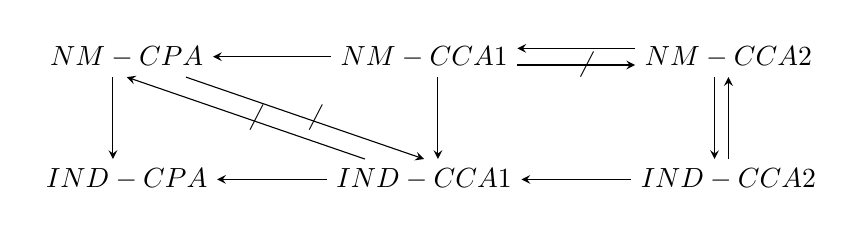
\begin{tikzpicture}
    \matrix (m) [matrix of math nodes,row sep=3em,column sep=4em,minimum width=2em]
    {
      NM-CPA & NM-CCA1 & NM-CCA2 \\
      IND-CPA & IND-CCA1 & IND-CCA2 \\
    };
    \path[-stealth]
    (m-1-2) edge (m-1-1)
    ([yshift=0.3em]m-1-3.west) edge ([yshift=0.3em]m-1-2.east)
    (m-2-2) edge (m-2-1)
    (m-2-3) edge (m-2-2)
    ([xshift=-0.5em]m-1-1.south) edge ([xshift=-0.5em]m-2-1.north)
    ([xshift=0.5em]m-1-2.south) edge ([xshift=0.5em]m-2-2.north)
    ([xshift=-0.5em]m-1-3.south) edge ([xshift=-0.5em]m-2-3.north)
    (m-1-1) edge node {$\not$} (m-2-2.north)
    (m-2-2) edge node {$\not$} (m-1-1.south)
    (m-2-3) edge (m-1-3)
    ([yshift=-0.3em]m-1-2.east) edge node {$\not$} ([yshift=-0.3em]m-1-3.west);
      \end{tikzpicture}
  \caption{All relations between our defined security frameworks. See Section
    \ref{sec:allrelations} for the explanation of the arrows.}
  \label{fig:secrelations}
\end{figure}
\subsection{Issues with deterministic schemes}
\begin{theorem}
  \label{thm:determ_enc_insecure}
  Let $\Pi = (\Gen, \Enc, \Dec)$ be a (stateless) cipher, such that $\Enc$ is deterministic.
  Then $\Pi$ cannot be IND-atk secure.
\end{theorem}
\begin{proof}
  All we need is the encryption oracle in stage 1, which we do under every
  threat model, since we are assuming that the publick key and $\Enc$ are known
  to the adversary. Therefore, construct a $\PPT$ adversary $\A$ as follows:
  \begin{algorithmic}
    \State \textbf{Algorithm} $\A$ \textbf{Stage 1}
    \State $m_0, m_1 \leftarrow \M$.
    \State Calculate $c_i = \Enc_{pk}(m_i)$ for $i \in \{0, 1\}$
    \State \Return $(m_0, m_1)$
    \State
    \State \textbf{Algorithm} $\A(c)$ \textbf{Stage 2}
    \If{$c = c_0$}{ \Return 0 }\Else{ \Return 1} \EndIf
    \State
  \end{algorithmic}
  Since $\Enc$ is deterministic, $m_0, m_1$ will always be encrypted to $c_0,
  c_1$, respectively. This means that $\A$ will guess correctly with probability 1,
  and hence $\Pi$ is not IND-atk secure.
\end{proof}
\begin{corollary}
  \label{cor:determ_nm_insecure}
  Let $\Pi = (\Gen, \Enc, \Dec)$ be a (stateless) cipher, such that $\Enc$ is deterministic.
  Then $\Pi$ cannot be NM-atk secure.
\end{corollary}
\begin{proof}
  Assume $\Pi$ is NM-atk secure. By Theorem \ref{thm:nm_imply_ind} we have that
  $\Pi$ is IND-atk secure, but since $\Enc$ is deterministic, by Theorem \ref{thm:determ_enc_insecure} we have
  that $\Pi$ cannot be IND-atk secure, a contradiction. Hence, our initial
  assumption must be false.
\end{proof}
\subsection{Security under multiple encryptions}
\paragraph{} The reader might find that we focused solely on the case when the
adversary is only observing a single ciphertext, and may wonder if it is perhaps
unrealistic to only consider this simple case. Luckily, it can be shown that \textit{goal-atk}
security under a single encryption implies \textit{goal-atk} security under
\textbf{multiple} encryptions. Formalising the notion of multiple encryptions
takes some effort and proving the above claim is non-trivial, however, we will
only acknowledgeme the result and not prove it. For a rigorous treatment see
Section 11 in \cite{katz2014introduction} (in particular Theorem 11.6).
\section{Public-Key Crypto Schemes}
\paragraph{} When one first encounters the concept ciphers it is tempting to believe that
the only way of obfuscated information exchange may only work if the method that
decrypts some text is the ``inverse'' of the method that was used to encrypt it.
The analogy being here that a cipher is a ``chest'' into which the honest
parties can place their information and ``lock'' it and ``unlock'' it with the
same key. Indeed, this general belief was held until quite recently, until the
groundbreaking work of Diffie and Hellman \cite{diffie1976new} and Rivest,
Shamir and Adleman \cite{rivest1978method}. They introduced the concept of
asymmetric encryption, where, continuing with the chest analogy, the party who
wished send a message could still place the message in the chest, however, they
would lock it with a padlock (the public key) and only the receiving party would
have the key to the padlock (the private key). Formally, this meant that the
secret key could not be obtained from the public key in polynomial time with
better than negligible probability. Next, we will discuss this idea and then
give a basic example of an asymmetric cipher.
\subsection{Hardness assumptions}
\label{sec:hardness_assumptions}
\paragraph{} All asymmetric schemes rely on certain assumptions about computing
values of some functions with or without the knowledge of some secret piece of
information is either ``easy'' or ``hard''. We will call such functions
\textbf{trapdoors} or \textbf{trapdoor functions}. The idea then is use the
function without the secret to perform encryption and use its inverse with the
secret to decrypt. Sadly, we do not have space for a
full formal discussion on these objects (namely one-way functions, trapdoor
functions and hard-core predicates). For a rigorous treatment, see Chapter 7 in \cite{katz2014introduction}.
Instead, we focus on exposing a few examples, to which we will come back in
later sections.
\paragraph{} The way we will approach defining our hardness assumptions will be
familiar to the reader: it is in the same vein as our definitions of security
frameworks! In particular, we will rely on the notion of experiments. Thus, we
begin with our first experiment:
\begin{definition}{The Factoring Experiment} The factoring experiment
  $\Expr{factor}{\A, \GenModulus}(n)$ involving a $\PPT$ adversary $\A$ and
  $\PPT$ algorithm $\GenModulus$ is as follows:
  \begin{enumerate}
  \item We run $\GenModulus(1^n)$, obtaining the tuple $(N, p, q)$, with $p, q$
    primes, $|p| = |q| = n$ and $N = pq$.
  \item $\A$ is given $N$, and outputs some $p', q' > 1$.
  \item We set $\Expr{factor}{\A, \GenModulus}(n) = 1$ if $p'q' = N$ and $0$ otherwise.
  \end{enumerate}
\end{definition}
There are two details in the above definition that are currently unclear: do
there always exist two primes of equal (binary) length and does such a
$\PPT$ algorithm $\GenModulus$ exist? Luckily for us the answer to both
questions is ``yes''. The first follows from the (improved) Bertrand-Chebyshev
theorem. As for the second problem, one such algorithm uses the so-called
\textit{Miller-Rabin prime test}, which runs
in polynomial time in $n$ and fails with negligible probability $\negl(n)$. For
a detailed discussion on $\PPT$ prime testing, see Chapter 3 Section 4 in \cite{hoffstein2014introduction}.
Now, we can formally define the factoring assumption:
\begin{definition}{The Factoring Assumption}
  Factoring is hard relative to $\GenModulus$ if for all $\PPT$ adversaries $\A$
  we have
  \[
    \Prob(\Expr{factor}{\A, \GenModulus}(n) = 1) \leq \negl(n).
  \]
\end{definition}
Essentially, the above definition says that factoring gets very hard as the
length of the primes used increases. Although this problem has been known and
studied for a very long time, it does not yield a straightforward trapdoor.
Instead, we will rely (for now) on the following experiment and hardness assumption:
\begin{definition}{The RSA Experiment}
The RSA experiment $\Expr{RSA-inv}{\A, \GenRSA}(n)$ involving a $\PPT$ adversary $\A$ and
  $\PPT$ algorithm $\GenRSA$ is as follows:
  \begin{enumerate}
  \item We run $\GenRSA(1^n)$, obtaining the tuple $(N, e, d)$
  \item We choose uniformly a $y \leftarrow \Int_N^*$.
  \item $\A$ is given $N, e, y$, and outputs some $x \in \Int_N^*$.
  \item We set $\Expr{RSA-inv}{\A, \GenRSA}(n) = 1$ if $x^e = y \mod N$ and $0$ otherwise.
  \end{enumerate}
\end{definition}
  We have our experiment, now we can define our assumption:
  \begin{definition}{The RSA Assumption}
    \label{def:rsa_assumption}
  The RSA problem is hard relative to $\GenRSA$ if for all $\PPT$ adversaries $\A$
  we have
  \[
    \Prob(\Expr{RSA-inv}{\A, \GenRSA}(n) = 1) \leq \negl(n).
  \]
\end{definition}
\paragraph{} Now, crucially, we will relate the RSA assumption to the factoring
assumption, meaning we can rely on the hardness assumption of a much better
studied problem. To do this, we will now show how to obtain the algorithm
$\GenRSA$ from $\GenModulus$. Therefore, consider the following algorithm:
\begin{algorithm}
  \begin{algorithmic}
    \State $\GenRSA(1^n):$
    \State $(N, p, q) \leftarrow \GenModulus(1^n)$
    \State $\phi(N) := (p - 1)(q - 1)$
    \State Choose $e > 1$ such that $\gcd(e, \phi(N)) = 1$
    \State Compute $d := e^{-1} \mod N \quad$ (note $e^{-1} \mod N$ exists since
    by the above step $e \in \Int^*_N$) 
    \State \Return $(N, e, d)$
    \State
  \end{algorithmic}
  \caption{GenRSA using GenModulus}
  \label{alg:genrsa}
\end{algorithm}
Therefore, we can now say that the RSA assumption holds, as long as the
factoring assumption does! The great thing about the RSA assumption, however, is
that it will give us a really nice trapdoor, that we will present in the next
part of this section.
\subsection{The RSA cryptoscheme}
\subsubsection{Mathematical set-up}
\begin{theorem}{Order}
  Let $G$ be a finite group and $g \in G$. Then, there exist positive integers
  $n$ such that $g^n = 1$. We shall call the smallest such integer the order of
  $g$, denoted $|g|$ called the \textbf{order} of $g$.
\end{theorem}
\begin{proof}
  Since $G$ is finite, there must exist $n, m \in \Nat, n \neq m$ such that
  \[
    g^n = g^m.
  \]
  Without loss of generality, we may assume $n > m$. Then, multiplying both
  sides with the inverse of $g^m$, we get
  \[
    g^{n - m } = 1.
  \]
\end{proof}
\begin{theorem}
  \label{thm:elemorderdiv}
  Let $G$ be a finite group and $g \in G$. Then, the order of $g$ divides the
  order of $G$.
\end{theorem}
\begin{proof}
  Assume that $|g| \nmid |G|$. Then, $|G| = q|g| + r$ for $q$ a non-negative
  integer and $r$ a positive integer.
\end{proof}
\begin{corollary}
  \label{cor:elemgroupordpow}
  Let $G$ be a finite group. Then,
  \[
    \forall g \in G\quad g^{|G|} = 1.
  \]
\end{corollary}
\begin{proof}
  Let $g \in G$. By Theorem \ref{thm:elemorderdiv} $|G| = q|g|$ for some $q \in
  \Nat$. Therefore,
  \[
    g^{|G|} = g^{q|g|} = (g^{|g|})^q = 1^q = 1.
  \]
\end{proof}
\begin{corollary}
  \label{thm:groupordpow}
  Let $G$ be a finite group. Then,
  \[
    \forall g \in G, p \in \Nat\quad g^p = g^{p \mod |G|}.
  \]
\end{corollary}
\begin{proof}
  \label{thm:grouppowmod}
  Let $g \in G, p \in \Nat$. Then, $p = q|G| + r$ for $q$ non-negative integer
  and $r$ a positive integer. Then, by the previous corollary $g^{|G|} = 1$, so
  \[
    g^p = g^{q|G| + r} = (g^{|G|})^qg^r = 1^qg^r= g^r = g^{p \mod |G|}.
  \]
\end{proof}
Before we may move on to the final corollary, we quickly make the following
observation:
\begin{theorem}
  Let $n \in \Nat$. The elements $x$ of $\Int_n \setminus \{0\}$ such that $\gcd(x, n) = 1$ form
  a group under multiplication with identity $1$ and inverse $a \in \Int_n$,
  where $ax + bn = 1$ from B\`ezout's identity. We denote this group by $\Int^*_n$
\end{theorem}
\begin{proof}
  It is very easy to check that the above indeed fulfils all group axioms.
\end{proof}
The order of $\Int_n$ is very important number-theoretically, so much so that it
is usually dentoted $\phi(n) = |\Int_n|$ and is called the \textbf{Euler phi-function}.
Now, we are ready to state the theorem of our interest:
\begin{theorem}{(Euler's Theorem)}\\
  \label{thm:eulersthm}
  Let $a, n \in \Nat$ such that $a < n$ and $\gcd(a, n) = 1$. Then,
  \[
    a^{\phi(n)} = 1 \mod n.
  \]
\end{theorem}
\begin{proof}
  By the above conditions $a \in \Int^*_n$. Then, the statement is a special
  case of Corollary \ref{thm:groupordpow}, where $(G, \circ) = (\Int^*_n, \times)$.
\end{proof}
\subsubsection{The Construction: RSA}
\paragraph{}
We are now ready to construct the well-known RSA scheme invented by Rivest,
Shamir and Adleman in 1978 \cite{rivest1978method}. As mentioned above, computationally secure schemes rely on
a security parameter $\lambda \in \Nat$. Increasing it will make the scheme run
slower, but will also make it more resilient. 
\paragraph{}
We first look at the trapdoor that we wish to use. We will take the function $f_e:
\Int_N \to \Int_N$ defined by
\[
  f_e: m \mapsto m^e \mod N 
\]
for some $e \in\Nat$.
It is clear that $f$ may be computed in polynomial time for arbitrary $e$. From Definition
\ref{def:rsa_assumption} and its following discussion that using an appropriate
$\GenModulus$, inverting $f$ is hard. However, if $d = e^{-1} \mod N$ is known,
inverting $f$ becomes easy. (See below for a proof of this.)
\paragraph{Key generation}
Run $(N, e, d) \leftarrow\GenRSA$ as defined in Algorithm \ref{alg:genrsa}. Set
$pk = (N, e)$ and $sk = (N, d)$ and output $(pk, sk)$.
\paragraph{Encryption}
Our message and cipher space are the binary string representations of naturals such that $m
< N$. Formally, $\M = \C = \{0, 1\}^{\lfloor {\log_2N} \rfloor}$.
\begin{enumerate}
\item Given public key $(N, i)$ and message $m \in \M$ calculate $c = m^i \mod N$.
\item Output $c$.
\end{enumerate}
\paragraph{Decryption}
\begin{enumerate}
\item Given private key $(N, j)$, and ciphertext $c \in \C$ calculate $m'''''''''= c^j \mod
  N$.
\item Output $m'$.
\end{enumerate}
\paragraph{Correctness} To show that the above scheme is indeed a cipher, we
must show that it is correct, i.e. that
\[
  \forall (k_\Enc, k_\Dec) \in \K, \forall m \in \M\quad\text{we have}\quad
  \Dec_{k_\Dec}(\Enc_{k_\Enc}(m)) = m.
\]
To see this, let $k_\Enc = (N, i)$ and $k_\Dec = (N, j)$ such that $(k_\Enc,
k_\Dec) \in \K$ and let $m \in \M$ be arbitrary. Then,
\[
  c = \Enc_{k_\Enc}(m) = m^i \mod N.
\]
Decrypting, we get
\begin{align*}
  m'' &= \Dec_{k_\Dec}(c) \\
     &= c^j \mod N \\
     &= (m^i)^j \mod N = m^{ij} \mod N \\
     &= m^{ij \mod N} \mod N \quad \text{by Corollary \ref{thm:grouppowmod}} \\
     &= m^1 \mod N \quad \text{Since $j$ is the multiplicative inverse of $i$ mod $N$ by definition}
\end{align*}
Since $m < N$ we may omit the mod $N$ on the last line. Therefore m = m' and so the scheme is correct.
\subsubsection{Security of RSA}
\paragraph{} Our construction above is what is usually referred to as ``textbook
RSA'' since it presents the cipher's underlying mechanism in its purest form,
with all technical improvements stripped away. Sadly, this also means that in
the security framework we set up, our construction is insecure. In particular, we note that
$\Enc$ is deterministic and that $\Pi$ is stateless, hence by Theorem
\ref{thm:determ_enc_insecure} and Corollary \ref{cor:determ_nm_insecure} our
construction is insecure in every security framework. This issue has been first
pointed out by Goldwasser and Micali in \cite{goldwasser1984probabilistic}. 
\paragraph{} However, the above does not mean that RSA is useless, in fact,
quite the contrary. Under some (reasonable) assumptions an improved version of
RSA using a method called Optimal Asymmetric Encryption Padding (OAEP) can be
proven to be IND-CCA2 secure. See Section 11.5 in \cite{katz2014introduction}
for a detailed discussion on the matter.
\section{Homomorphic Crypto Schemes}
\paragraph{}
At this point, we start to finally focus on the topic of the dissertation:
homomorphic schemes. Intuitively, these encapsulate the idea of encrypted
comptutation over encrypted data, in sense that the adversary may at most
observe the operation take place, but both the inputs and the output of it
remain secret. In this section we give the formal definition, construct an
example scheme known as the Paillier scheme. Finally, we close with a discussion
on the limitation of homomorphic schemes.
\subsection{What is homomorphic encryption?}
\subsubsection{The definition}
\begin{definition}{Homomorphic Cipher}
  Let $\Pi = (\Gen, \Enc, \Dec)$ be a cipher with message space $\M$ and cipher
  space $\C$. Furtermore, let $(\M, \circ)$ and $(\C, \oplus)$ be groups where
  $\circ, \oplus$ are binary operations.
  We say that $\Pi$ is homomorphic iff $\forall (k_\Enc, k_\Dec) \in \K, \forall
  m_1, m_2 \in \M, c_1 = \Enc_{k_\Enc}(m_1), c_2 = \Enc_{k_\Enc}(m_2)$ we have
  \[
    m_1 \circ m_2 = \Dec_{k_\Dec}(c_1 \oplus c_2).
  \]
\end{definition}
\subsubsection{Limitations}
\paragraph{} The reader may not yet see the advantages of homomorphic schemes,
however, one aspect will be clear immediately: these ciphers are
\textit{extremely} malleable. We formalise this in the theorem below:
\begin{theorem}
  Let $\Pi = (\Gen, \Enc, \Dec)$ be a homomorphic cipher. Then $\Pi$ cannot be
  secure in the NM-atk sense. 
\end{theorem}
\begin{proof}
  We prove the above claim by exhibiting a $\PPT$ adversary $\A$ which breaks
  NM-atk security with non-negligible advantage. Concretely, define $\A$ as
  follows:
  \begin{algorithmic}
    \State \textbf{Algorithm} $\A$ \textbf{Stage 1}
    \State Pick $M := \M \setminus \{1_\M\}$ such that $M$ samples uniformly,
    i.e. every element has a $\frac1{|\M| - 1}$ chance of being picked.
    \State \Return M
    \State
    \State \textbf{Algorithm} $\A(c)$ \textbf{Stage 2}
    \State Calculate $c'' = c \oplus c$.
    \State \Return $(c', R)$ where $R$ is the quadratic residue relation, i.e. $R(a,
    b) = True$ iff $a \circ a = a^2 = b$.
    \State
  \end{algorithmic}
  Let $m, \textbf{m}'$ as defined in the NM-atk security experiment. We note
  that in our case we have $\textbf{m}' = \Dec_{sk}(c \oplus c) = m \circ m =
  m^2$, where the penultimate equality follows, since $\Pi$ is a homomorphic cipher. 
  \paragraph{Claim} $m \not\in \textbf{m}'$. \\
  The above is equivalent to stating that $m \neq m^2$. Assume the contrary,
  i.e. that $m = m^2$. Since $\M$ is a group, we have inverses. Multiplying by
  $m^{-1}$ on both sides then, we get $1_\M = m$, which is impossible by the
  definition of $\A$, hence our claim holds.
  \paragraph{}
  Since $\textbf{m}' = m^2$, we have $R(m, \textbf{m}') = True$ for any input.
  Putting this together with our claim above, we have that $\A$ succeeds with
  probability 1, hence clearly $\A$ has non-negligible advantage, thus $\Pi$
  is not NM-atk secure.
\end{proof}
Now, the reader may assume that this must mean that the highest security level a
homomorphic cipher may obtain is IND-CPA security. However, this assumption is
not true! In particular, recall Section \ref{sec:security_frameworks} Figure
\ref{fig:secrelations}, based on the results of \cite{bellaresecurityrelations}.
We see that IND-CCA1 does not imply NM-CPA security, leaving open the
possibility of IND-CCA1 secure homomorphic ciphers. A somewhat surprising recent
result result is achieved by Yasuda et al. \cite{Yasuda2018}, where they construct a
cipher where in fact the relationship between the message and the cipherspace is
a ring homomorphism, and they show that their scheme is IND-CCA1 secure!
\subsection{Paillier's Scheme}
\paragraph{}
Here we will give a concrete example of a homomorphic scheme, called the Paillier
cryptosystem, named after Pascal Paillier, who invented it in 1999
\cite{paillier1999public}. Once again, however, before we discuss the
construction of the scheme, we must familiarize ourselves with the theory upon
which it is built.
\subsubsection{Mathematical Set-up}
The cryptosystem is built on a particular isomorphism between two groups, that
we will be proving here. However, before we can do that, we revisit the $\phi$
function.
\begin{theorem}
  \label{thm:phiformula}
  Recall that Euler's $\phi$-function is defined as
  \[
    \phi(N) = |\{k \in \{0\hdots N - 1\} \,\,|\,\, \gcd(k, N) = 1\}|
  \]
  Assume $N = \prod_{i = 1}^n p_i^{e_i}$, for $p_i$ primes and $e_i$ naturals. Then,
  \[
    \phi(N) = \prod_{i = 1}^n p_i^{e_i - 1} (p_i - 1).
  \]
\end{theorem}
\begin{proof}
  We will present a simple counting argument using the inclusion-exclusion
  principle. That is, let $\P$ be the set of prime divisors of $N$, and
  let $\D_P$, where $P \subseteq \P$ be the set of integers
  between $0$ and $N - 1$ divisible by all primes in $P$. Formally:
  \[
    \text{For } P \subseteq \P \quad \D_P = \{n \in \{0 \hdots
    N - 1\}\,\,|\,\,p | n\,\,\forall p \in P\}.
  \]
  Then, our problem can be reformulated in the following way:
  \[
    \phi(N) = |\D_\emptyset|.
  \]
  We observe the following two simple facts: First
  \[
    |\D_P| = \frac{|N|}{\prod_{p \in P}p} = \prod_{i = 1}^n p_i^{e_i -
      1} \times \prod_{p \not\in P}p
  \]
  Second, for any $A = \{a_1, a_2, \hdots a_n\}$ integers we have
  \begin{equation}
    \label{eq:prodexpansion}
    \prod_{i = 1}^n (a_i - 1) = \sum_{i = 0}^n (-1)^i
 \sum_{\substack{B \subseteq A \\ |B| = n - i}} \prod_{a \in B}a
  \end{equation}
  This holds, because if we expand the left-hand term, then every term in the
  result will be a product of $n - k$ first terms and $k$ second terms. The
  expression on the right hand merely captures summing all possible combinations.
  By the inclusion-exclusion principle we have
  \begin{align*}
    |\D_\emptyset| &= |\{0 \hdots N-1\}| - \sum_{\substack{P \subseteq \P \\ |P| =
        1}} |\D_P| + \sum_{\substack{P \subseteq \P \\ |P| =
        2}} |\D_P| - \hdots \sum_{\substack{P \subseteq \P \\ |P| =
    |\P|}} |\D_P| \\
                   &= N + \sum_{i = 1}^n (-1)^i \sum_{\substack{P \subseteq \P \\ |P| =
    i}} |\D_P| \\
                   &= N + \sum_{i = 1}^n (-1)^i \sum_{\substack{P \subseteq \P \\ |P| =
        i}} \left(  \prod_{i = 1}^n p_i^{e_i - 1} \times \prod_{p \not\in P}p \right)\\
                   &= \prod_{i = 1}^n p_i^{e_i - 1} \left( \prod_{p\in\P}p +  \sum_{i = 1}^n (-1)^i \sum_{\substack{P \subseteq \P \\ |P| =
    i}} \prod_{p \not\in P}p \right) \quad \text{merge the product with the sum}\\
                   &= \prod_{i = 1}^n p_i^{e_i - 1} \left( \sum_{i = 0}^n (-1)^i
 \sum_{\substack{P \subseteq \P \\ |P| = n - i}} \prod_{p \in P}p \right) \quad\text{by Equation \ref{eq:prodexpansion}}\\
                   &=\prod_{i = 1}^n p_i^{e_i - 1}\prod_{p \in \P} (p - 1) = \prod_{i = 1}^n p_i^{e_i - 1}(p_i - 1).
 \end{align*}
\end{proof}
\paragraph{Note:} A much nicer proof of the above result follows from Chinese
Remainder Theorem using the fact that for $m, n \in \Nat$ where $\gcd(m, n) = 1$
we have $\phi(mn) = \phi(m)\phi(n)$, but this is outside the scope of this work. 
\begin{theorem}
  \label{thm:paillierthms}
Let $1^n$ be our security parameter. Let $p, q$ be primes such that
$|p| = |q| = n$ and $N = pq$. Then, the following hold:
\begin{enumerate}
\item $\gcd(N, \phi(N)) = 1$
\item For any $a \in \Int_{N^2}^*$ we have $(1 + N)^a = 1 + aN \mod N^2$. In
  particular, the order of $1 + N$ is $N$.
\item We have $\Int_{N^2}^* \cong \Int_{N} \times \Int_{N}^*$.
In particular, the isomorphism $f:\Int_{N} \times \Int_{N}^* \mapsto \Int_{N^2}^*$
is given by
\[
   f((a, b)) = (1 + N)^a \times b^N \quad\text{for}\,\, a \in \Int_{N}, b \in \Int_{N}^*.
\]
\end{enumerate}  
\end{theorem}
\paragraph{Claim 1:} We may assume without loss of generality, that $p > q$.
Then obviously $\gcd(p, p - 1) = 1$ and $\gcd(p, q - 1) = 1$. If $\gcd(q, p - 1)
\neq 1$, then $\gcd(q, p - 1) = q$, since $q$ is a prime. But then $p - 1 = aq$
for some $a \in \Nat$, in particular $\frac{p - 1}{2} \geq q$ from which $|p| >
|q|$, a contradiction, hence $\gcd(q, p - 1) = 1$. From this we have $\gcd(q,
\phi(N)) = 1$ and $\gcd(p, \phi(N)) = 1$ and therefore $\gcd(N, \phi(N)) = 1$.
\paragraph{Claim 2:} Expanding $(1 + N)^a$ by the binomial theorem, we get
\[
  (1 + N)^a = \sum_{i =0}^a \binom{a}{i} N^i
\]
Reducing modulo $N^2$, all terms with degree 2 or higher become 0 and the only
two terms remaining will be $1 + aN$. From this, setting $a = N$ we get $(1 +
N)^N = 1$, and this is the smallest possible positive integer.
\paragraph{Claim 3:}
For clarity, we shall follow the notation of \cite{katz2014introduction} and
write
\[
  (a, b) \leftrightarrow x \Leftrightarrow f((a,b)) = x
\]
\begin{proof}
  We shall break down the proof into the following steps:
  \begin{enumerate}[i.]
  \item Show $f$ is a bijection.
  \item Show $f$ is a homomorphism.
  \end{enumerate}
  \paragraph{Claim 3.i} We first note the following:
  \[
    |\Int_{N}| = N = pq,\quad
    |\Int_{N}^*| = \phi(N) = (p - 1)(q - 1),\quad
    |\Int_{N^2}^*| = \phi(N^2) = pq(p - 1)(q - 1),
  \]
  where the last two equalities hold by Theorem \ref{thm:phiformula}.
  This means that since $|\Int_{N} \times \Int_{N}^*| = |\Int_{N}|
  \times |\Int_{N}^*|$ we have $|\Int_{N} \times \Int_{N}^*| = |\Int_{N^2}^*|$.
  Hence, we only need to show that $f$ is a injection to show that it is a bijection.
  \paragraph{}
  Therefore, let $f((a_1, b_1)) = f((a_2, b_2))$ for some $(a_1, b_1), (a_2,
  b_2) \in \Int_{N} \times \Int_{N}^*$. Then,
  \[
    (1 + N)^{a_1}\times b_1^N = (1 + N)^{a_2}\times b_2^N\mod N^2
  \]
  Then, since we have inverses in both $\Int_N$ and $\Int_N^*$, we have
  \[
    (1 + N)^{a_1 - a_2}\times (b_1b_2^{-1})^N = 1 \mod N^2
  \]
  Since $b_1, b_2 \in \Int_N^*$, raising both sides to the power of $\phi(N)$,
  we get
  \begin{align*}
    (1 + N)^{\phi(N)(a_1 - a_2)} \times ((b_1b_2^{-1})^{\phi(N)})^N &= 1 \mod N^2 \\
    (1 + N)^{\phi(N)(a_1 - a_2)}  &= 1 \mod N^2\quad\text{by Corollary \ref{cor:elemgroupordpow}}
  \end{align*}
  Then, since by Claim 1 $\gcd(N, \phi(N)) = 1$, it must be the case that $(1 +
  N)^{a_1 - a_2} = (1 + (a_1 - a_2)N) = 1 \mod N^2$. Hence $a_1 - a_2 = 0 \mod N^2$
  and since $a_1, a_2 \in \Int_N$ the above is an equality, from which we have
  $a_1 = a_2$.
  \paragraph{} Going back to our initial formula, now simplifying by the terms
  involving the $a$s:
  \[
    b_1^N = b_2^N \mod N^2.
  \]
  Since $b_1, b_2 \in \Int_N^*$ we have $b_1, b_2\in \Int_{N^2}^*$. But
  exponentiation in finite groups is a bijection, hence $b_1 = b_2 \mod N^2$.
  Again, since $b_1, b_2 < N$, it is actually an equality. Thus $f$ is
  injective, and hence bijective.
  \paragraph{Claim 3.ii} Let $a_1, a_2 \in \Int_N$ and $b_1, b_2 \in \Int_N^*$. We need to show that
  \[
    f((a_1, b_1)) \times f((a_2, b_2)) = f((a_1 + a_2), (b_1b_2)).
  \]
  We note that the multiplication on the left-hand side is carried out modulo
  $N^2$, whereas the addition and multiplication on the right-hand side is done
  modulo $N$. We will begin with
  \begin{align*}
    (1 + N)^{a_1}b_1^N(1 + N)^{a_2}b_2^N &= (1 + N)^{a_1 + a_2}(b_1b_2)^N \mod N^2 \\
                                         &= (1 + N)^{[a_1 + a_2 \mod N]}(b_1b_2)^N \mod N^2 \quad \text{by Claim 2 and Theorem \ref{thm:grouppowmod}}
  \end{align*}
  The addition is now carried out modulo $N$, but there is some more work with
  the multiplication. Let $b_1b_2 = \gamma N + r$ where $0 \leq \gamma$ and $0 <
  r \leq N$. Note that $r \neq 0$, since that would mean $b_1b_2$ is divisible
  by $N$, but it is not since it is in $\Int_N^*$. Then, by the Binomial
  Theorem, we have
  \begin{align*}
    (b_1b_2)^N &= (\gamma N + r)^N \\
               &= \sum_{i = 0}^N \binom{N}{i}(\gamma N)^ir^i \\
               &= r^N \mod N
  \end{align*}
  This means that $(b_1b_2)^N$ is an Nth power modulo $N$, and hence $f$ is a
  homomorphism. \\
  By Claim 3.i and Claim.ii, $f$ is an isomorphism.
\end{proof}
Finally, we look at the particular set of elements used in Paillier's scheme:
$N$th residues.
\begin{definition}{Nth residue:} Let $G$ be a group and let $x, y \in G$. Then, we call $y$
  an Nth residue, if $x^N = y$, and write $y \in \texttt{Res}(G)$.
\end{definition}
We now characterise Nth residues in $\Int_{N^2}^*$.
\begin{theorem}
  Let $x \in \texttt{Res}(\Int_{N^2}^*)$ be an Nth residue. Then, $\exists b \in
  \Int_N^*$ such that
  \[
    x \leftrightarrow (0, b),
  \]
  and thus
  \[
    \texttt{Res}(\Int_{N^2}^*) = \{b \,\,|\,\, b \in \Int_N^*\}.
  \]
\end{theorem}
\begin{proof}
  We will construct a generic Nth residue. Let $a \in \Int_N$ and $b \in
  \Int_N^*$. By Claim 1, $\gcd(N, \phi(N)) = 1$, hence $N$ has a multiplicative
  inverse mod $\phi(N)$. Call this inverse $d = N^{-1}$. Then, $b^d$ is also in $\Int_N^*$. Then, let $x \in \Int_{N^2}^*$ such
  that
  \[
    x \leftrightarrow (a, b^d).
  \] 
  Note, that since $a$ and $b$ were arbitrary and $f$ is an isomorphism, every
  element of $\Int_{N^2}^*$ can be written in the above form. Raising both sides
  to the Nth power, we get
  \begin{align*}
    x^N &\leftrightarrow (a, b^d)^N \\
        &\leftrightarrow (aN \mod N, b^{dN} \mod N) \\
        &\leftrightarrow (0, b).
  \end{align*}
\end{proof}
\paragraph{} We also note that it is easy to see from the above that there are
precisely $N$ elements mapping to the same residue, since all elements of the
form $(a, b^d)$ map to $(0, b)$, and since $a\in \Int_N$, there are $N$ choices
for $a$. However, this means that sampling $\Int_{N^2}^*$ uniformly means that
we are sampling \texttt{Res}($\Int_{N^2}^*$) uniformly too!
\paragraph{} Finally, in this section we consider a new hardness assumption:
   \begin{definition}{The Decisional Composite Residuosity Problem (DCRP):} The
     DCRP is hard relative to $\GenModulus$ if for all $\PPT$ adversaries $\A$
     we have
     \[
       \left| \Prob(\A(N, [r^N amod N^2]) = 1) - \Prob(\A(N, r) = 1) \right|
       \leq negl(n)
     \]
     where we run $(N, p, q) \leftarrow\GenModulus(1^n)$ and the pick $r$
     uniformly from $\Int_{N^2}^*$.
   \end{definition}
   Essentially, the DCRP states that for the appropriate $\GenModulus$ deciding
   if we picked an Nth residue or we sampled the whole group uniformly is hard.
\paragraph{} Now, we have all the tools required to construct the scheme.
\subsubsection{The Construction: Paillier Cryptoscheme}
\paragraph{} As with RSA, we first expose the trapdoor we will be using. Define
$f_y: \Int_N \to \Int_{N^2}^*$ by
\[
  f_y: m \mapsto (1 + N)^m \cdot y \mod N^2 
\]
for some $y \in \Int_N^*$. Again, it is clear that computing $f$ can be
performed in polynomial time for arbitrary $y$. However, by the DCRP assumption
$f$ is hard to invert, since we would need to invert $y \in \texttt{Res}(N^2)$
to be able to calculate $m$ from $f(m)$. However, if we are given $\phi(N)$,
inverting $f$ becomes easy! (See below for proof.)
\paragraph{Key Generation}
Pick two primes of length equal to the security parameter, i.e. $p, q$ primes,
such that $|p| = |q| = |\lambda|$. Calculate $N = pq$, $N^2$ and $\phi(N) = (p -
1)(q - 1)$.
Then output $pk = N^2$ and $sk = \phi(N)$.
\paragraph{Encryption}
Let $m$ be the message we wish to encrypt. Pick a uniform $(0, r) \in
\Int_{N^2}^*$. Then output the ciphertext $c = (m, 1) \times (0, r) = (m, r)$.
\paragraph{Decryption} 
Let $c$ be the ciphertext we wish to decrypt. First, let $\hat{c} = c^{\phi(N)}
\mod N^2$. Then, calculate $m' = \frac{(\hat{c} - 1)}{N} \times \phi(N)^{-1} \mod N$.
Output $m'$.
\paragraph{Correctness}
Let $(pk, sk)$ be the key $\Gen$ generates, with $pk = N^2$, for some $N = pq$
primes and $sk = \phi(N)$. Let$m$ be the message we encrypt and $c =
\Enc_{pk}(m) =(m, r)$ for some uniformly random $r$. Then
\begin{align*}
  \hat{c} &= c^{\phi(N)} = (m, r)^{\phi(N)} = (\phi(N)m, r^{\phi(N)}) \\
          &= (\phi(N)m, 1) \quad \text{by Corollary \ref{cor:elemgroupordpow}}\\
          &\leftrightarrow (1 + N)^{\phi(N)m} \mod N^2 \quad \text{by Theorem \ref{thm:paillierthms} part 2}\\
          &= (1 + \phi(N)mN) \mod N^2.
\end{align*}
Then, we have
\begin{align*}
  \Dec_{sk}(c) &= \frac{\hat{c} - 1}{N} \times \phi(N)^{-1} \mod N\\
               &= \frac{(1 + \phi(N)mN) - 1}{N} \times \phi(N)^{-1} \mod N\\
               &= \frac{\phi(N)mN}{N}\times \phi(N)^{-1} \mod N\\
               &= \phi(N)m \times \phi(N)^{-1} \mod N \\
               &= m \mod N. \\
               &= m \quad \text{since } m < N.
\end{align*}
Thus, $m = \Enc_{pk}(\Dec_{sk}(m))$, and so the scheme is correct, and therefore
a cipher.
\subsubsection{The security of our construction}
\paragraph{} Here we show that Paillier encryption is IND-CPA secure.
\begin{theorem}
  Let $\Pi = (\Gen, \Enc, \Dec)$ as in Paillier's scheme. If the DCRP assumption
  holds with respect to $\GenModulus$, then $\Pi$ is IND-CPA secure.
\end{theorem}
\begin{proof}
  Let $\A$ be an arbitrary $\PPT$ adversary. We will now define a $\PPT$
  algorithm $\A'$ such that it attempts to solve DCRP with $\A$ as a subroutine,
  with respect to $\GenModulus$.
  Hence, define $\A'$ as
  \begin{algorithmic}
    \State \textbf{Algorithm} $\A'(N, y)$
    \State Obtain $(m_0, m_1) \leftarrow \A$ Stage 1
    \State Generate a bit $b \in \{0, 1\}$ uniformly.
    \State Compute $c = (1 + N)^{m_b} \cdot y \mod N^2$.
    \State Set $b' = \A(c)$ Stage 2.
    \State \Return $1$ if $b = b'$ and $0$ otherwise.
    \State
  \end{algorithmic}

We will now analyse the behaviour of $\A'$ under the two possibilities that may
happen in the DCRP.
\paragraph{Case 1.} We ran $(N, p, q) \leftarrow \GenModulus(1^n)$, chose an $r
\in \Int_{N^2}^*$ uniformly and set $y = r^N \mod N^2$. Then, we called $\A'(N,
y)$. \\
Here we will be passing $c = (1 + N)^{m_b} \cdot r^N \mod N^2$ to the second
stage of $\A$. Since here we will have $c = \Enc(m_b)$, by the definition of the
indistinguishability experiment we will have
\[
  \Prob(\Expr{ind-cpa}{\Pi, \A} = 1) = \Prob(\A \text{ outputs } b | B = b) =
  \Prob(\A'(N, [r^N \mod N^2]) = 1).
\]
\paragraph{Case 2.} We ran $(N, p, q) \leftarrow \GenModulus(1^n)$, chose an $r
\in \Int_{N^2}^*$ uniformly and set $y = r$. Then, we called $\A'(N, y)$.
Here, since $y$ is just uniformly picked from the ambient group, the output of
$\A$ does not depend on $b$. Hence $\Prob(\A'(N, r) = 1) = \frac12$.
\paragraph{} By the DCRP assumption, we have
\[
  \left| \Prob(\A'(N, [r^N \mod N^2]) = 1) - \Prob(\A'(N, r) = 1) \right| \leq \negl(n).
\]
By the two above case analyses we get
\[
\left| \Prob(\Expr{ind-cpa}{\Pi, \A} = 1) - \frac12 \right| \leq \negl(n)
\]
and hence
\[
  \Adv{ind-cpa}{\Pi, \A} = 2 \cdot \Prob(\Expr{ind-cpa}{\Pi, \A} = 1) - 1 \leq \negl(n).
\]
Thus, $\Pi$ is IND-CPA secure.
\end{proof}
\section{Lattices}
\paragraph{}
In the previous section we have seen the motivating idea behind Gentry's scheme:
encrypted computation. In this section, we aim to provide a brief introduction
to the tool that helped the scheme come to life: lattices. We will define what a
lattice is and see some key definitions and theorems. We will close the section
with a construction of a simple lattice-based crypto scheme to illustrate how
the theory may be used to construct secure schemes with the appropriate choice
of a trapdoor. \cite{hoffstein2014introduction}
\subsection{Mathematical Set-up I: Vector Spaces and Rings}
\paragraph{} As it happens, lattices and then later a special species of them
that will be of particular interest to us rely on the theory of vector
spaces and rings. Therefore, we first review these structures. We note that
these may be defined in a very general sense, however, we shall focus on
definitions involving only the real numbers.
\subsubsection{Vector Spaces}
\paragraph{} We begin with vector spaces. These will enable us to formalise a
lot of geometric arguments very neatly. Thus, we begin with their definition.
\begin{definition}{Vector Space:}
  Let $V \subseteq \Reals^n$ for some $n \in \Nat$. Then, we say that $V$ is a
  vector space iff for all $\vec{v}_1, \vec{v}_2 \in V$ and $\alpha_1, \alpha_2
  \in \Reals$ we have
  \[
    \alpha_1\vec{v}_1 + \alpha_2\vec{v}_2 \in V.
  \]
\end{definition}
We immediately follow up with 3 key definitions involving members of $V$.
\begin{definition}{Linear Combination:}
  Let $V$ be a vector space, and $W = \{\vec{v}_1, \hdots, \vec{v}_m\} \subseteq
  V$. Then, a linear combination of the vectors in $W$ is the vector
  \[
    \vec{w} = \alpha_1\vec{v}_1 + \hdots + \alpha_m\vec{v}_m\quad\text{ with }
    \alpha_1, \hdots \alpha_m \in \Reals.
  \]
  The set of all combinations that can be made up using the vectors in $W$ is
  called the \textbf{span} of $W$. Formally:
  \[
    \Span(W) = \{\vec{w} = \alpha_1\vec{v}_1 + \hdots + \alpha_m\vec{v}_m
    \,\,|\,\, \alpha_1, \hdots \alpha_m \in \Reals, \vec{v}_1,\hdots, \vec{v}_m
    \in W \}.
  \]
\end{definition}
\paragraph{} One can think of the span of a set of vector as the ``smallest''
space in which all vectors related to the elements of $W$ can be found.
Geometrically, it is the ``smallest'' set of points that can be reached from the
origin by translating by scaled version of the vectors in $W$. It is usually
convenient to collect vectors in $W$ in a structured way, called a matrix. If we
collected the scaling factors in a vector $\vec{\alpha} = (\alpha_1, \hdots,
\alpha_m)$, then we can express the vector $\vec{w}$ by writing
\[
  \vec{w} = \vec{\alpha} \cdot W = \vec{\alpha} \cdot 
  \begin{bmatrix}
    - \vec{v}_1 - \\
    \vdots \\
    - \vec{v}_m - 
  \end{bmatrix}
\]
\begin{definition}{Linear Independence}
  Let $V$ be a vector space, and $W = \{\vec{v}_1, \hdots, \vec{v}_m\} \subseteq
  V$. We say that the vectors of $W$ are linearly independent if
  \[
    \vec{0} = \alpha \cdot W\quad\text{ with }
    \vec{\alpha} = [\alpha_1, \hdots \alpha_m] \in \Reals^m 
 \]
  holds if and only if $\alpha_1 = \alpha_2 = \hdots = \alpha_m = 0$. If the
  condition does not hold, we call the vectors of $W$ linearly dependent.
\end{definition}
\paragraph{} Geometrically, one can think of linearly independent vectors as
vectors not parallel to each other.
\begin{definition}{Basis}
  Let $V$ be a vector space, and $W = \{\vec{v}_1, \hdots, \vec{v}_m\} \subseteq
  V$. Then, we say $W$ is a basis for $V$ if we have $\Span(W) = V$ and the
  vectors of $W$ are linearly independent.
\end{definition}
\begin{theorem}
  Let $V$ be a vector space. Then, $V$ has a basis, and for any bases $B_1, B_2$
  we have $|B_1| = |B_2|$. We call this unique number the dimension of $V$ and
  write $\dim(V) = |B_1|$.
\end{theorem}
\paragraph{} We now briefly discuss the idea of projecting a vector onto
another, as well as measuring the length of a vector or the distance between two
vectors.
\begin{definition}{Inner product:}
  Let $\vec{u} = [u_1, \hdots, u_n], \vec{v} = [v_1, \hdots, v_n] \in \Reals^n$.
  Then define the inner product of $\vec{u}, \vec{v}$ as
  \[
    \vec{u} \cdot \vec{v} = \sum_{i = 1}^n u_iv_i.
  \]
\end{definition}
On can think of the inner product of two vectors as the ``generalised'' length
of the shadow (projection) of one vector on the other.
We can then use the length of the projection of a vector onto itself as a way of
measuring its length. In particular:
\begin{definition}{Norm}
  Let $\vec{v} = [v_1, \hdots, v_n] \in R^n$. Then we say that the (Euclidean) norm (length) of
  $\vec{v}$ is defined as
  \[
    \norm{\vec{v}} = \sqrt{\vec{v} \cdot \vec{v}} = \sqrt{v_1^2 + \hdots + v_n^2}.
  \]
\end{definition}
Finally, using the definition of length, we may measure distance between any two
vectors by measuring the length of their difference:
\begin{definition}
  Let $\vec{v}, \vec{u} \in \Reals^n$. Then, the (Euclidean) distance between
  them is defined as
  \[
    d(\vec{v}, \vec{u}) = \norm{v - u}.
  \]
\end{definition}
\paragraph{} We note here that all the definitions above fulfil the axioms of
inner product space theory, normed space theory and metric space theory,
respectively. We also note that the norm and the metric we are imposing on
$\Reals^n$ are exactly the norm and metric induced by the inner product.
Finally, we finish with an important geometric concept: perpendicular lines.
In a generalised setting we will say that two vectors are perpendicular to each
other if the length of the shadow of one on the other is $0$. Formally:
\begin{definition}
  Let $\vec{v}, \vec{u} \in \Reals^n$. We say that they are orthogonal
  (perpendicular) to each other if we have
  \[
    \vec{v} \cdot \vec{u} = 0.
  \]
\end{definition}
\subsubsection{Rings}
\paragraph{} The theory of rings is a very rich subject with many different
applications, for our purposes, however, after the initial abstract definition
will only focus on polynomial rings. We thus begin with some basic definitions:
\begin{definition}{Ring:}
  Let $R$ be a commutative group under some binary operation $+$ with identity
  element $0$. Then, let $\times: R \setminus \{0\} \to R \setminus \{0\}$ be a
  binary operation. We say that $(R, +, \times)$ is a ring (we will later just
  refer to $R$ being a ring, implicitly implying the tuple) if the following
  hold:
  \begin{itemize}
  \item \textbf{R1:} $\forall x, y, z \in R$ we have 
    \[
      (x \times y) \times z = x \times (y \times z)\quad  \text{(associativity)}
    \]  
  \item \textbf{D:} $\forall x, y z \in R$ we have 
    \[
      x \times (y + z) = x \times y + x \times z \quad\text{and}\quad (x + y) \times z = x \times z + y \times z \quad\text{(distributivity)}
    \] 
 \end{itemize}
\end{definition}
Often it is convenient to talk about the set of the ring $R$ with the additive
identity removed. Thus, henceforth we shall write $R^* = R \setminus \{0\}$ to
avoid clutter.
\begin{definition}{Field:}
  Let $(F, +, \times)$ be a ring. If $(F^*, \times)$ forms an
  commutative group, we say $F$ is a field.
\end{definition}
\begin{definition}{Ideal:}
  Let $R$ be a ring and $I \subseteq R$ with the following three properties:
  \begin{itemize}
  \item \textbf{I1:} $I \neq \emptyset\quad$ (non-emptiness) 
  \item \textbf{I2:} $\forall a, b \in I$ we have
      \[
        a + b \in I\quad\text{(closure under ring addition)}
      \]
    \item \textbf{I3:} $\forall i \in I, r \in R$ we have
      \[
        r \times i \in I\quad\text{and}\quad i \times r \in I\quad\text{(ideal property)}
      \]
  \end{itemize}
\end{definition}
We then have a very natural way of obtaining an ideal, using a set of elements
from $R$:
\begin{definition}{Generators}
  Let $S = \{i_1, \hdots, i_n\} \subseteq R$. Then, we say that the ideal
  \textbf{generated by} $S$ is
  \[
    I = (S) = \{r_1i_1 + \hdots + r_ni_n \,\,|\,\, r_1, \hdots, r_n \in R\}.
  \]
  If $S = \{i\}$ is a singleton set, we write $I = (i)$ and say that $I$ is a
  \textbf{principal ideal}.
\end{definition}
\begin{definition}{Modding by an ideal:}
  \label{def:ideal_mod}
  Let $R$ be a ring and $I$ an ideal of $R$. Let $\pi + I$ be a coset of $I$ and
  $\psi \in \pi + I$. Assume that $\pi$ is in some sense a unique ``special''
  element. We will call $\pi$ a \textbf{distinguished representative} of $I$.
  Then, we will define
  \[
    \psi \mod I := \pi.
  \]
\end{definition}
\begin{definition}{Sum of ideals}
  Let $R$ be a ring and $I$, $J$ be ideals in $R$. Then, we can define a new set
  \[
    I + J = \{i + j \,\,|\,\, i \in I, j \in J\}.
  \]
  Then, $I + J$ is again an ideal of $R$.
\end{definition}
\begin{definition}{Relatively prime ideals}
  Let $R$ be a ring and $I$, $J$ be ideals in $R$. Then, we say that $I$ and $J$
  are relatively prime, iff
  \[
    I + J = R.
  \]
\end{definition}
\paragraph{Example} For the ring of integers $R = \Int$ the ideal of even numbers
$I = (2)$ and the ideal of numbers divisible by 5 $J = (5)$ are relatively
prime, i.e. $(2) + (5) = (1) = \Int$.
\begin{definition}{Quotient Ring:}
  Let $R$ be a ring and $I$ be an ideal of $R$. Then, the set
  \[
    R/I = \{r + I\,\,|\,\, r \in R\}
  \]
  Forms a ring under the additive operation $+: R/I\times R/I \to R/I$ defined by
  \[
    \forall (r_1 + I), (r_2 + I) \in R/I\quad (r_1 + I) + (r_2 + I) = (r_1 +
    r_2) + I \in R/I
  \]
  and the multiplicative operation $\times: R/I\times R/I \to R/I$ defined by
  \[
    \forall (r_1 + I), (r_2 + I) \in R/I\quad (r_1 + I) \times (r_2 + I) = (r_1 \times
    r_2) + I \in R/I,
  \]
  called the quotient of $R$ modulo $I$, and the elements of $R/I$ are called
  the cosets of $I$.
\end{definition}
It can be shown that the cosets of $I$ are either the same or disjoint.
\begin{definition}{(Univariate) Polynomial Ring over $R$:}
  Let $R$ be a ring. Then, define a \textbf{polynomial of degree $m$ in $x$ with
  coefficients in $R$} as
\[
  p(x) = r_0 + r_1x + r_2x^2 + \hdots + r_mx^m
\]
where $r_0,\hdots, r_m \in R$ are the coefficients of $p$. We call the $x^i$
the powers of $x$, and we call the highest power of $x$ the degree of the
polynomial. Now, define the set of all finite degree polynomials over $R$ by
\[
  R[x] = \bigcup_{i = 0}^\infty \left\{p(x) = \sum_{j = 0}^i r_jx^i\,\,|\,\,r_j \in R\quad
  \forall 0 \leq j \leq i\right\}.
\]
Then, the set $R[x]$ forms a ring under the additive operation $+: R[x]\times
R[x] \to R[x]$ defined by
\[
  \forall p(x) = \sum_{i = 0}^n p_ix^i, q(x) = \sum_{i = 0}^m q_ix^i \in
  R[x]\quad p(x) + q(x) = \sum_{i = 0}^{\max(m, n)} (p_i + q_i)x^i
\]
where the missing $p_is$ or $q_is$ are just assumed to be $0$, and under the
multiplicative operation $\times: R[x]\times
R[x] \to R[x]$ defined by
\[
  \forall p(x) = \sum_{i = 0}^n p_ix^i, q(x) = \sum_{i = 0}^m q_ix^i \in
  R[x]\quad p(x) \cdot q(x) = \sum_{i = 0}^{m + n} c_ix^i
\]
where
\[
  c_i = \sum_{\substack{0 \leq k, l \leq m + n \\ k + l = i}} p_kq_l.
\]
\end{definition}
Finally, we consider some concepts which arise from the number theoretic origins
of rings.
\begin{definition}{Unit}
  Let $R$ be a ring, that has a multiplicative identity. Then, we say that an
  element $u \in R^*$ is a unit, iff it has a multiplicative inverse in $R^*$
\end{definition}
\begin{definition}{Divisibility}
  Let $R$ be a ring and $r, s \in R$. Then, we say that $s$ \textbf{divides}
  $r$, iff there is some $t \in R$, such that $r = st$. We call $(s,t)$ a
  \textbf{divisor pair}.
\end{definition}
\begin{definition}{Irreducibility}
  Let $R$ be a ring with a multiplicative identity. Then, we say that an element
  $r \in R^*$ is irreducible if $r$ is not a unit and all of its divisor pairs have a unit in them. In other
  words, if we have $r = uv$ for some $u, v \in R$, then either $u$ or $v$ is a unit.
\end{definition}
\subsection{Mathematical Set-up II: Introduction to Lattices}
\label{sec:lattice_intro}
\paragraph{} We shall begin by a basic introduction to lattices in general, then
turn our attention to computational problems involving lattices. In the
following section, we construct a very simple cryptosystem that relies on the
ideas we explore here.
\begin{definition}{(Finite dimensional) Lattice:}
  Let $V = \Reals^n$ be the $n$-dimensional Euclidean space, and $B = \{\vec{v}_1,
  \vec{v}_2, \hdots, \vec{v}_n\}$ be a basis for $V$. Then, the \textbf{lattice generated by $B$} is the set
  \[
    \L(B) = \{\alpha_1\vec{v}_1 + \alpha_2\vec{v}_2 + \hdots \alpha_n\vec{v}_n\,\,|\,\, \vec{v}_i \in B,
    \alpha_i \in \Int\}.
  \]
  Then $B$ is also called the basis of the lattice $\L$.
\end{definition}
\begin{definition}{Fundamental Domain}
  Let $\L$ be a lattice with basis $B = \{\vec{v}_1, \vec{v}_2, \hdots, \vec{v}_n\}$. Then, the
  \textbf{fundamental domain of $\L$ with respect to $B$} is
  \[
    \F_B = \{t_1\vec{v}_1 + t_2\vec{v}_2 + \hdots + t_n\vec{v}_n \,\,|\,\, \vec{v}_i \in B, t_i \in [-\frac12,
    \frac12)\} \subseteq \Reals^n.
  \]
\end{definition}
The following theorem is key for cryptographic application of lattices:
\begin{theorem}
  Let $\L$ be a lattice with basis $B$. Then $\F_B$ tessalates $\Reals^n$
  without overlap. Formally, let $x \in \Reals^n$. Then there exists a unique $\ell \in \L$
  and $f \in \F_B$ such that
\[
  x = \ell + f.
\]
\end{theorem}
\begin{proof}
  Let $x \in \Reals^n$ be arbitrary. Since $B = \{ \vec{v}_1, \hdots, \vec{v}_n \}$ is a basis for $\Reals^n$, there
  is a unique combination of its vectors that give $x$, i.e. there exist unique
  reals $a_1, \hdots, a_n$ such that
  \[
    x = a_1\vec{v}_1 + \hdots + a_n\vec{v}_n.
  \]
  For all $i$ let $\alpha_i = \lfloor a_i \rceil$ and $t_i = a_i - \lfloor a_i
  \rceil$. We note that by the definition of the round function, $-\frac12 \leq t_i <
  \frac12$ for all $i$. Then, letting $\ell = \sum_{i = 1}^n \alpha_i\vec{v}_i$ and $f
  = \sum_{i = 1}^n t_i\vec{v}_i$, we clearly have $\ell \in \L$ and $f \in
  \F_B$. Now, from the above equation we get
  \begin{align*}
    x &= (\alpha_1 + t_1)\vec{v}_1 + \hdots (\alpha_n + t_n)\vec{v}_n \\
      &= \alpha_1\vec{v}_1 + \hdots + \alpha_n\vec{v}_n + t_1\vec{v}_1 + \hdots + t_n\vec{v}_n \\
      &= \ell + f \quad \text{as required.}
  \end{align*}
\end{proof}
We can use the above result we make the following observation: given a point in
a lattice $\L(B)$'s ambient space $\vec{v} \in \Span(B)$, we can ``distil''
it's offset. We can write up $\vec{v} = \ell + \vec{f}$ for some $\ell\in
\L(B)$ and $f \in \F(B)$, then calculate
\[
  \vec{v}\times B^{-1} = (\ell + \vec{f}) \times B^{-1} = \ell\times B^{-1} +
  \vec{f}\times B^{-1}.
\]
Since $\ell = \vec{a} \times B$ and $\vec{f} = \vec{t} \times B$ for $\vec{a}
\in \Int^n$ and $\vec{t} \in \left[-\frac12, \frac12\right)^n$, from the above we have
\[
  \vec{v}\times B^{-1} = \vec{a} + \vec{t}.
\]
Now, since $\vec{a}$ is an integer vector, the entire fractional part must come
from $\vec{t}$. Thus rounding both sides, since every entry in $\vec{t}$ rounds
to 0 by its definition, we get
\[
  \lfloor \vec{v}\times B^{-1} \rceil = \lfloor \vec{a} + \vec{t} \rceil = \vec{a}.
\]
Hence, we define the following:
\begin{definition}{Modding by a lattice basis}
  \label{def:lattice_mod}
  \begin{align*}
    \vec{v} \mod B &= \vec{v} - \lfloor \vec{v} \times B^{-1} \rceil \times B \\
                   &= \ell + \vec{f} - \vec{a} \times B \\
                   &= \ell + \vec{f} - \ell = \vec{f}.
  \end{align*}
\end{definition}
This gives a really nice way of testing whether a point in the ambient space is
also in the lattice, since if $\vec{v} \in \L(B)$, then $\vec{v} \mod B = 0$!
\begin{definition}
  Let $\L$ be an $n$-dimensional lattice with basis $B$ and fundamental domain
  $\F_B$. Then, the $n$-dimensional volume of $\F_B$ is called the determinant
  (or covolume) of $\L$, denoted by $\det(\L)$.
\end{definition}
\begin{theorem}
  \label{thm:lattice_change_of_basis}
  Let $\L$ be a lattice with bases $B_1, B_2$. Then, there exists a matrix $A$
  with $\det(A) = \pm 1$ such that $AB_1 = B_2$.
\end{theorem}
\begin{proof}
\end{proof}
\begin{theorem}{Hadamard's inequality}
  Let $\L$ be a lattice with basis $B = \{\vec{v}_1, \vec{v}_2, \hdots \vec{v}_n\}$. Then
\[
  \Vol(\L) \leq \norm{\vec{v}_1}\cdot\norm{\vec{v}_2}\cdots\norm{\vec{v}_n}.
\]
\end{theorem}
Based on the above theorem, we will make the following definition:
\begin{definition}{Hadamard Ratio}
  Let $\L$ and $B$ as in the theorem above. Then, the \textbf{Hadamard ratio of $B$}
  is defined as
  \[
    \H(B) = \left( \frac{\Vol(\L)}{\norm{\vec{v}_1}\cdot\norm{\vec{v}_2}\cdots\norm{\vec{v}_n}} \right)^{\frac1n}.
  \]
\end{definition}
We note that by the above theorem $0 < \H(B) \leq 1$.
\begin{theorem}
  Let $\L$ be a lattice with basis $B = \{v_1, \hdots, v_n\}$. Then, $Vol(\F_B) = |\det(B)|$
\end{theorem}
\begin{proof}
  We clearly have
  \[
    \Vol(\F_B) = \int_{\F_B} dx_1dx_2\cdots dx_n.
  \]
  We do not know much about the variables $x_i$, so using the defintion of the
  fundamental domain, we change the variables of the integration:
  \[
    \vec{x} = \vec{t} \cdot B
  \]
  where $\vec{x} = [x_1, \hdots x_n] \in \Reals^n, \vec{t} = [t_1, \hdots, t_n] \in
  [0, 1)^n$. Then, the Jacobian of the above equation if $B$.
  Note, that $[0, 1)^n = C_n$ is the $n$-dimensional unit cube, and
  hence $C_n$ is precisely the pre-image of $\F_B$ under the map $B$. Hence, $BC_n = \F_B$.
  Therefore, changing the variables, we will have
  \begin{align*}
    \int_{\F_B} dx_1dx_2\cdots dx_n &= \int_{BC_n} dx_1dx_2\cdots dx_n =
                                      \int_{C_n} |\det(B)|dt_1dt_2\cdots dt_n \\
                                    &= |\det(B)|\Vol(C_n) = |\det(B)|.
  \end{align*}
\end{proof}
\begin{corollary}
  Let $\L$ be a lattice with bases $B_1, B_2$. Then, $\det(\L)$ is independent
  of its bases.
\end{corollary}
\begin{proof}
  By Theorem \ref{thm:lattice_change_of_basis}, there is a matrix $A$ such that
  $\det(A) = \pm 1$ and
  \[
    AB_1 = B_2.
  \]
  Then, from the definition of covolume, we have
  \begin{align*}
    \Vol(\F_{B_1}) &= |\det(B_1)| \\
                  &= |\det(A)| \cdot |\det(B_1)| \\
                  &= |\det(AB_1) | \\
                  &= |\det(B_2)| \\
                  &= \Vol(\F_{B_2}).
  \end{align*}
\end{proof}
\subsubsection{Ideal Lattices}
\label{sec:ideal_lattices}
We now approach the final (and possibly most complicated) object that we will
require for our constructions: ideal lattices. These are the objects that will
possess structure under two operations, while at the same time have a nice
geometric interpretation, and yield an efficient trapdoor. To see their
connection to rings and how they are constructed, we show the following theorem.
\begin{theorem}{Ideal membership in integer polynomial fields:}
 Let $f \in \Int[x]$ be an irreducible polynomial of degree $n$. Let $R = \Int[x]/f$. Then, an
 element $p(x) = p_1 + \hdots + p_nx^n\in R$ is a polynomial of degree at most $n$, and hence it may be
 represented by a vector $\vec{p} = [p_1, \hdots p_n] \in \Int^n$. Define the \textbf{rotation
   basis} of $p$ by
 \[
   P =
   \begin{bmatrix}
     p_1 & p_2 & \cdots & p_n \\
     -p_n & p_1 & \cdots & p_{n - 1} \\
     \vdots & & & \vdots \\
     -p_2 & -p_3 & \cdots & p_n
   \end{bmatrix}
 \]
 Then, a polynomial $q(x) \in R$ is in the ideal $(p(x))$ if and only if its
 corresponding coefficient vector $\vec{q} \in \Int^n$ is in the lattice $\L(P)$. 
\end{theorem}
\begin{proof}
  We show that the claim is implied in both directions.
  \paragraph{Forward direction:} $q(x) \in (p(x)) \Rightarrow \vec{q} \in \L(P)$.\\
  $q(x) \in (p(x))$ means that there is some $v(x) \in R$ such that $q(x) = v(x)
  \times p(x)$. In particular, we will thus have integers $a_0, \hdots a_n$ such that
  \[
    q(x) = \sum_{i = 0}^n a_ip(x)x^i \mod f(x)
  \] which corresponds precisely with
  $\vec{a} \cdot P \in \L(P)$. Hence $\vec{q} \in \L(P)$.
\paragraph{} We observe that all of the above steps are reversible, hence \textbf{the
backwards direction} holds as well.
\end{proof}
The above if and only if condition motivates the following definition.
\begin{definition}{Ideal Lattice:}
  Let $R, p$ and $P$ be as in the above theorem. Then, we call $\L(P)$ the ideal
  lattice induced by $p$.
\end{definition}
The above definition is made to really highlight the dual nature of the ideal $(p)$.
\paragraph{} Finally, we draw attention to the two modding operations that we
have defined: modding a ring element by an ideal in Definition
\ref{def:ideal_mod} and modding an element of $n$-dimensional Euclidean space by
a lattice basis in Definition \ref{def:lattice_mod}. The question now arises: since ideal
lattices are related to both rings and lattices, is there a connection between
the two operations? The answer is not only that the two are related, but they
are exactly the same operation! (Hence, when we later write mod in the context of
ideal lattices, it will not be an overload of notation.) To see that they are
equal, we observe the following: Since an element in $R$ may be represented as a
vector in $\Int^n$, given an ideal $(v(x))$ and another ring element $a(x) \in
R$, we have
\[
  a(x) \in p(x) + (v(x)) \quad\Leftrightarrow\quad \vec{a} \in \vec{p} + \L(V)
  \quad\Leftrightarrow\quad \vec{a} = \vec{p} \mod V
\]
where $V$ is the rotation basis corresponding to $v(x)$.
\subsection{Mathematical Set-up III: Computational Considerations for Lattices and Rings}
\paragraph{} Up to now, we only considered structures in the context of the
properties that their axioms give rise to. In this section, we now switch
context, and consider them from a computational point of view. In particular,
we consider computational problems that arise from lattices that can be used to
construct public-key ciphers.
\subsubsection{Computational Lattice Problems}
\label{sec:comp_lattice_prob}
\begin{definition}
  Let $\L$ be a lattice. Then, define $\lambda_i(\L)$ called the $i$th
  successive minimum of $\L$ as the smallest radius $r > 0 $ such that $\L$
  contains at least $i$ linearly independent (non-zero) vectors with norm at most $r$.
\end{definition}
The reader should think about the above definition as a ball around the origin
with the smallest such radius that (at least) $i$ non-collinear points fall in
the ball. In particular, the ball with radius $\lambda_1(\L)$ will only contain
one point, the shortest vector in $\L$. (Actually, the ball may contain more
than one point as long as they all have the same norm.)
\begin{definition}{The $\gamma(n)$-SVP Experiment} The SVP experiment
  $\Expr{SVP}{\A, \GenBasis}(n)$ with factor $\gamma(n)$ involving a $\PPT$ adversary $\A$ and
  $\PPT$ algorithm $\GenBasis$ is as follows:
  \begin{enumerate}
  \item We run $\GenBasis(1^n)$, obtaining the tuple $(P, S)$, with $P, S \in
    \GL_n(\Rat)$ such that there exists a unimodular matrix $U$ with integer
    coefficients (i.e. $U \in \GL_n(\Int)$ with $|\det(U)| = 1$) such that $US =
    P$.
  \item $\A$ is given $P$, and outputs some $\vec{v} \in \L(P)$.
  \item We set $\Expr{SVP}{\A, \GenBasis}(n) = 1$ if $\vec{v} \leq \gamma(n)
    \cdot \lambda_1(\L(P))$ and $0$ otherwise.
  \end{enumerate}
\end{definition}
\begin{definition}{$\gamma(n)$-Shortest Vector Problem (SVP) Assumption}
  $\gamma(n)$-SVP is hard relative to $\GenBasis$ if for all $\PPT$ adversaries $\A$ we
  have
  \[
    \Prob(\Expr{SVP}{\A, \GenBasis}(n) = 1) \leq \negl(n).
  \]
\end{definition}
\begin{definition}{The $\gamma(n)$-CVP Experiment} The CVP experiment
  $\Expr{CVP}{\A, \GenCVP}(n)$ with factor $\gamma(n)$ involving a $\PPT$ adversary $\A$ and
  $\PPT$ algorithm $\GenCVP$ is as follows:
  \begin{enumerate}
  \item We run $\GenCVP(1^n)$, obtaining the tuple $(\vec{w}, P, S)$, with $P, S \in
    \GL_n(\Rat)$ such that there exists a unimodular matrix $U$ with integer
    coefficients (i.e. $U \in \GL_n(\Int)$ with $|\det(U)| = 1$) such that $US =
    P$ and $\vec{w} \in \Span(P)$.
  \item $\A$ is given $P$ and $\vec{w}$, and outputs some $\vec{v} \in \L(P)$.
  \item We set $\Expr{CVP}{\A, \GenCVP}(n) = 1$ if $\norm{\vec{v} - \vec{w}} \leq \gamma(n)
    \cdot \norm{\vec{v} - \vec{u}}$ for any other $\vec{u} \in \L(P)$ and $0$ otherwise.
  \end{enumerate}
\end{definition}


\begin{definition}{$\gamma(n)$-Closest Vector Problem (CVP) Assumption}
   $\gamma(n)$-CVP is hard relative to $\GenCVP$ if for all $\PPT$ adversaries $\A$ we
  have
  \[
    \Prob(\Expr{CVP}{\A, \GenCVP}(n) = 1) \leq \negl(n).
  \]
\end{definition}
\paragraph{} There are two details that are currently unclear. Firstly, are
there $\PPT$ algorithms $\GenBasis$ and $\GenCVP$ as specified in the above
definitios, with respect to which our hardness assumptions hold? Secondly, is
there a connection between CVP and SVP so that we can base the hardness
assumption of one problem on the assumption of the other (as we did with the
factoring and RSA assumptions in Section \ref{sec:hardness_assumptions})? The answer in both
questions is fortunately ``yes''. In particular, Ajtai shows in
\cite{AjtaiLatticeAvgWorst} that essentially solving average-case (i.e. randomly
generated instances of) SVP is polynomially equivalent to solving a different,
worst-case lattice problem, the Short Basis Problem (SBP). In the framework of
this text, this means for us that the SBP yields a $\PPT$ algorithm $\GenBasis$
with respect to which our SVP assumption holds. As for the connection between
CVP and SVP, they can both be reduced into each other with the lattice dimension
of the problems changing at most very slightly after the reduction. See the
paper by Goldreich et al. for the SVP to CVP reduction \cite{GOLDREICH199955}
and Section 6.5 in \cite{hoffstein2014introduction} for the other direction as
well as a discussion on connections between other lattice problems. Again,
interpreting this within our framework, we can base our CVP hardness assumption
on $\GenBasis$ also.
\paragraph{} An interesting other approach relies on the idea of modding a
vector by a lattice basis that we saw in Section \ref{sec:lattice_intro}. We define the
following algorithm:
\begin{algorithm}[H]
  \caption{}
  \label{alg:babais_alg}
  \begin{algorithmic}
    \State On input $\vec{v}, B$
    \State Calculate $\vec{u} = \vec{v} - (\vec{v} \mod B)$
    \State \Return $\vec{u}$
  \end{algorithmic}
\end{algorithm}
Then, the vector $\vec{u}$ returned by Algorithm \ref{alg:babais_alg} is in $\L(B)$. Since
the input $\vec{v}$ is in the fundamental domain that surrounds $\vec{u}$, it is
certainly true that $\vec{v}$ is not very far from $\vec{u}$. In particular,
$\norm{\vec{v} - \vec{u}} \leq \norm{B}$. But how close are they actually? Is
$\vec{u}$ the closest lattice point to $\vec{v}$? If it is not in general, for
what bases of $\L$ is it? L\'aszl\'o B\'abai answered these questions in his
influential paper \cite{Babai1986} in 1983. He showed that for any lattice as long as vectors in $B$ are sufficiently
orthogonal to each other (Lov\'asz reduced, see \cite{lenstra1982factoring} for
precise details), then Algorithm \ref{alg:babais_alg} will indeed return the closest lattice
vector within an approximation factor of $\gamma(n) = 1 + 2n \cdot
(\frac92)^{n/2}$ where $n$ is the dimension of the lattice. However, if the
vectors in $B$ are not very orthogonal, there is a large number of lattice points that
are closer to $\vec{v}$ than $\vec{u}$. Due to these results, this algorithm is
named B\'abai's algorithm in his honour. What is great about this approach, is
not only does it put precise conditions on the parameters of the lattice, but it
immediately yields a trapdoor for a cipher: generate two bases for a lattice,
one with very orthogonal vectors, and another with quite parallel vectors in it,
and use them as our secret and public key, respectively. Then, a message can be
encoded using the public basis and can be recovered using the secret basis.
\subsubsection{Computational Ring Problems}
\paragraph{} In the above section we have seen concrete computational problems
involving lattices. We now take a step back, and consider two more abstract
problems, defined with rings. This approach will help us understand
relationships between the ciphers presented in this work. We begin with the
simpler one.
\begin{definition}{The Ideal Membership Experiment} The ideal membership experiment
  $\Expr{IMP}{\A, R, I, \Samp_I}(n)$ involving a $\PPT$ adversary $\A$, ring $R$, $I$ an
  ideal of $R$ and $\PPT$ algorithm $\Samp_I$ that samples from $I$
  according to some distribution is as follows:
  \begin{enumerate}
  \item We generate $r_0 \leftarrow \Samp_I$ and $r_1 \leftarrow R$ (uniformly).
    We also generate a bit $b \leftarrow \{0, 1\}$. 
  \item $\A$ is given $R, I, \Samp_I$ and $r_b$, and outputs some bit $b' \in \{0, 1\}$.
  \item We set $\Expr{IMP}{\A, \GenIdeal}(n) = 1$ if $b = b''''$ and $0$ otherwise.
  \end{enumerate}
\end{definition}
Hence, we are asking that given a ring $R$ and $I$ and some sampling function
$\Samp_I$, is it easy to determine if a randomly chosen element of $R$ is in
$I$. While this problem may seem very far removed from practicalities, we
consider the following two examples.
\paragraph{Example 1}
  Let $N$ be an integer such that it is a product of two primes of equal length.
  Then, set $R = \Int_N$ under addition and multiplication modulo $N$. Let $e$
  be a unit in $R$, and set $I = (e)$ and let $\Samp_I$ sample $I$ uniformly. Then,
  solving this instance of the IMP is exactly equivalent to solving the RSA
  problem. 
\paragraph{Example 2}
  Let $N = pq$ such that $p, q$ are primes of equal length. Set $R =
  \Int_{N^2}$, and set $I = (N)$ and let $\Samp_I$ sample $I$ uniformly. Then,
  noticing that $I = \texttt{Res}(N^2)$, solving this instance of the IMP is equivalent to solving the DCRP! Hence
  Paillier's scheme is also just a special case of the IMP.
\begin{definition}{Ideal Membership Problem (IMP) Assumption}
  IMP is hard relative to $(R, I, \Samp_I)$ if for all $\PPT$ adversaries $\A$ we have
  \[
    \Adv{IMP}{\A, R, I, \Samp_I}(n) = 2 \cdot \Prob(\Expr{IMP}{\A, R, I, \Samp_I}(n) = 1) - 1 = \negl(n)
  \]
\end{definition}
In ideal lattices, however, we are in trouble. It is because testing ideal
membership can be performed in polynomial time, in particular, given an ideal basis
$B_I$ and a vector $\vec{v} \in \L(B_I)$, it is enough to check if $\vec{v}
\mod B_I = 0$. Hence, if we wish to use ideal lattices as our source of hard
problems, we cannot use any that can be reduced into the IMP. This observation
motivates our second ring problem.
\begin{definition}{The Ideal Coset Experiment} The ideal coset experiment
  $\Expr{ICP}{\A, R, I, \Samp_R, \GenIdeal_I}(n)$ involving a $\PPT$ adversary $\A$, ring
  $R$, $I$ an ideal of $R$, $\PPT$ algorithm $\Samp_R$ that samples $R$
  according to some distribution and $\PPT$ algorithm $\GenIdeal$, assuming that modding by ideals may be performed
  in polynomial time, is as follows:
  \begin{enumerate}
  \item We run $\GenIdeal(1^n, R, I)$, obtaining the tuple $(J^{pk}, J^{sk})$,
    with $J^{pk}, J^{sk}$ generators of the same ideal $J$ in $R$.
  \item We generate $r_0 \leftarrow \Samp_R$ and $r_1 \leftarrow R$.
    We also generate a bit $b \leftarrow \{0, 1\}$. Then, we calculate $r = r_b
    \mod J^{pk}$.
  \item $\A$ is given $R, I, J^{pk}, \Samp_R$ and $r$, and outputs some bit $b' \in \{0, 1\}$.
  \item We set $\Expr{ICP}{\A, R, I, \Samp_R, \GenIdeal}(n) = 1$ if $b = b'$ and $0$ otherwise.
  \end{enumerate}
\end{definition}

\begin{definition}{Ideal Coset Problem (ICP) Assumption}
  The ICP is hard relative to $(R,I,\Samp_R,\GenIdeal)$ if for all $\PPT$ adversaries $\A$ we have
  \[
    \Adv{ICP}{\A, R, I, \Samp_R, \GenIdeal}(n) = 2 \cdot \Prob(\Expr{ICP}{\A, R,
      I, \Samp_R, \GenIdeal}(n) = 1) - 1 = \negl(n).
  \]
\end{definition}
\subsection{The Construction: GGH}
\paragraph{} To see the ideas presented above work in practice, we give a
straightforward application of them in a cryptosystem developed due to
Goldreich, Goldwasser and Halevi, named GGH in their honour \cite{goldreich1997public}.
\paragraph{Key Generation}
\paragraph{} Assume the security parameter is $\lambda = 1^n$. Generate a basis
$V \in \Int^{n\times n}$ with small Hadamard ratio. Then, generate a random matrix
$U \in \Int^{n\times n}$ such that $\det(U) = \pm 1$. Calculate $W = UV$. Output
$(pk, sk) = (W, U)$.
\paragraph{Encryption}
Let $pk = W$ and $m \in \Int^n$ be the message that we want to encrypt. Let $r
\in \Int^n$ be a random vector with $\norm{r}$ small. Then, caluclate and output
$c = mW + r$.
\paragraph{Decryption}
Let $pk = W$, $sk = V$ and $c$ the ciphertext we want to decrypt. Use Babai's
algorithm with $V$ and $c$ as inputs to obtain a vector $\hat{m} \in \Int^n$. Then multiply
$\hat{m}$ by $VW^{-1}$ on the right and output the answer.
\paragraph{Correctness}
Let $pk = W$, $sk = V$ and $m$ be the message we wish to encrypt. Then, $c =
\Enc_{pk}(m) = mW + r$, for some small $r$. Now, examining $\Dec_{sk}(c)$, we
find that first we calculate $\hat{m} = \lfloor cV^{-1} \rfloor$. Since $V$'s
Hadamard ratio is high we will have decoded to the closest lattice point, hence
we will now have $\hat{m}V = mW$. Hence by multiplying $\hat{m}$ by $VW^{-1}$ on
the left, we get
\[
  m'' = \hat{m}VW^{-1} = mWW^{-1} = m.
\]
Hence the cipher is correct.
\subsubsection{Security of GGH}
\paragraph{} IND-CPA
\section{Fully Homomorphic Encryption}
\paragraph{} At last, we have arrived at the crowning jewel of obfuscated
computation: \textbf{fully homomorphic encryption}, which will allow us to
compute the result of arbitrary functions on encrypted data! Here the author
aims to expose the core ideas that are involved in achieving such a scheme. Due
to its youth, there is rather limited literature available on the topic, hence
our narrative will be mostly following the footsteps of the inventor of the first
ever such scheme: the PhD thesis of Dr Craig Gentry \cite{gentry2009fully}.
Here, however, we run into a problem: the full description and justification of
the scheme draws on so many topics from different parts of mathematics, that
attempting to present the whole work would take a much longer work then this
one. Instead, our goal is to distil the core concepts and put them in the
context of what we already know. When this is not possible, we will point the
reader to the appropriate source.
\paragraph{}
This section takes a top-down approach to the explanation. That is, after the mathematical
preamble we will provide insight starting from the most abstract approach to the
concrete, implemented cipher. 
\subsection{Motivation, Definitions and Approach}
\label{sec:fhe_motivation}
\paragraph{}
We begin with a bunch of definitions that we will make use of later.
\paragraph{} Whenever one is designing a cipher, they would obviously want it to
be as quick as possible, whilst retaining security. In our case, as the reader
will see below this is an even more burning issue. For this reason, we look to
lattices as our solution, as the complexity of encryption and decryption
procedures which are yielded by their appropriate trapdoors in lattice based
schemes outperforms other currently known trapdoors and they are also better
parallelisable.
\paragraph{} This is complemented by the fact discussed in Section
\ref{sec:ideal_lattices}, that ideals in polynomial rings automatically
induce lattices. This dual nature of ideal lattices will immediately yield us
the ring homomorphisms between the message and the cipherspace that we need to
achieve FHE.
\paragraph{} However, there is an issue with lattices which we must patch: we
saw in Section \ref{sec:comp_lattice_prob} that checking ideal membership in
(ideal) lattices may be performed in polynomial time! In particular, all we need
to do is check for some $\vec{v} \in \L(B)$ for some lattice $\L$ with basis $B$
is whether $\vec{v} = 0 \mod B$. Therefore, we will rely on the slightly
different problem of the ideal coset problem (ICP), which will yield us a nice trapdoor.
\paragraph{} So how will all the above come together to give us FHE?
We first define a cipher that will be allow computation \textit{up to a certain
  level}. At this point, it is important to pause and identify the reason that
causes this limitation, because if the limitation is inherent to the scheme,
then any improvement upon it will be obviously futile. In our case, however, we
can ``tune'' the limitation, i.e. we can sacrifice computation time and memory
space to push our limitation further. In particular, our limitation will come
from the fact that the trapdoor the ICP in ideal lattices gives us is such that
each new ciphertext has some ``error'' associated with it (in particular it is the
coset representative) in which we embed our
message, that can be thought of as an offset from a lattice point. Then, adding
and multiplying ciphertexts will increase the error associated with their sum/
product, and at some point it grows so much that the offset will push the
ciphertext vector so far from its original lattice point that it will be closer
to another one, causing decryption failure. The question then is, can we
``reset'' this error somehow while preserving the correctness of the scheme.
The solution is to create a scheme that can evaluate a sufficiently complex
combination of operations so that it is capable of \textit{computing its own decryption function} (augmented with some operation at
the end)! The term we will use to describe a cipher with such a property is that
the cipher is \textbf{bootstrappable}.  Once we have a bootstrappable scheme, we
can use it to construct an (almost) fully homomorphic scheme! (The caveat being
that the length of the public key will depend on the complexity of the function
we wish to evaluate). Here is the core of the construction: Let $\Pi = (\Gen,
\Enc, \Dec)$ be a bootstrappable cipher. Let $m$ be our message and $c =
\Enc(pk_1, m)$ its encryption under some public key $pk_1$ (with corresponding
secret key $sk_1$).
\begin{enumerate}
  \item Calculate $c_0 = \Enc(pk_2, c) = \Enc(pk_2, \Enc(pk_1, m))$, the encryption of
    of $c$ under some public key $pk_2$.
  \item Calculate $c_1 = \Evaluate(\Dec, \{sk_1\, c_0\})$, i.e. we homomophically
  decrypt $c$ under $sk_1$. Hence, we will have $c_1 = \Enc(pk_2, m)$ (with
  some technical caveats).
\end{enumerate}
This is great, however, we have not made any progress, we just switched keys on
the encryption of $m$. This is why we will also require a bootstrappable cipher
to be able to evaluate its decryption function \textbf{together with some
  operation}. Hence, in step two we can actually call this augmented function
$\Dec^{op}$ with more than one ciphertext and make progress at the same time as
resetting the error.
\paragraph{} In the upcoming few sections, we will present the scheme that is
\textit{almost bootstrappable} (in Gentry's terminology, it is \textit{somewhat
  homomorphic}). This scheme, with some tweaks can then be made bootstrappable
and thus will yield us FHE.
\paragraph{}
Before we can move on, however, we are obliged to
clarify what we mean by being able to compute arbitrary functions on encrypted data.
What we will in fact show is that we are capable of evaluating arbitrary
(binary) circuits on ciphertexts. We will then rely on a theorem by Fischer
and Pippenger \cite{Fischer96lectureson}, which states that a \textit{family of circuits over a set functionally complete gates} can
simulate any Turing Machine. Then, by Church-Turing Thesis we have that we can
compute anything that is computable. We will now clarify functional
completeness:
\begin{definition}{(Informal) Functionally complete set:}
  Let $\Gamma$ be a set of boolean (binary) gates, such that every gate in the set is a
  binary operation, i.e $\forall g \in \Gamma$ we have $g: \{0, 1\} \times \{0,
  1\} \to \{0, 1\}$. Then, $\Gamma$ is functionally complete, if every Boolean
  function $f: \{0, 1\}^n \to \{0, 1\}$ may be expressed as a circuit of
  the elements of $\Gamma$. (Here the term circuit is left vague as it
  needs some care to define formally. The reader should think of it as the
  intuitive way of combining boolean gates.)
\end{definition}
Hence, all we need to show now is that our scheme can evaluate a functionally
complete set of gates. It is easy to show that given the function $\NAND(x, y)
\mapsto \neg (x \land y)$ the set $\{\NAND\}$ is functionally complete. The last
question remaining then is, how can we represent circuits in our scheme? To
answer this question, we need to know how the scheme works, so we will get the
answer to this question at the end of the next section.
\subsection{The Scheme, Abstractly}
\paragraph{} We are now going to present the somewhat homomorphic scheme that is
used to obtain a bootstrappable one. There are two reasons for presenting it
abstractly. Firstly, following our aim and convention in this work to present
the underlying mechanism of the cipher in its purest form, and secondly, because
we can base our security proofs on the abstract scheme. This means that if we
can ``substitute in'' more concrete objects that satisfy our assumptions, we
will not need to worry about security!
\subsubsection{Definition of the Scheme}
\paragraph{} For what follows, we will assume that given a ring $R$ and ideals
$I$ and $J$ of $R$, modding by the ideals may be performed in polynomial time.
\paragraph{Key Generation} We are given a security parameter $\lambda = 1^n$. We
generate a (description of) ring $R$ appropriate to $\lambda$. Also fix an ideal
$I$ in $R$. Now, run $\GenIdeal(\lambda, R, I)$, such that we obtain $(J^{pk},
J^{sk})$, such that $(J^{sk})$ and $I$ are relatively prime. Set $pk = (R, I,
J^{pk}, \Samp_R)$ as the public key and $sk = (R, I, J^{sk})$ as the secret key.
Output $(pk, sk)$.
\paragraph{Encryption} Given a public key $pk = (R, I, J^{pk}, \Samp_R)$ and a
message $m$ perform the following: calculate $c' = \Samp_R(I, m)$. Here,
$\Samp_R(I, m)$ samples an element from the coset $m + I$ in the ring $R/I$.
Then, calculate $c = c' \mod J^{pk}$. Output $c$.
\paragraph{Decryption} Given a secret key $sk = (R, I, J^{sk})$ and some
ciphertext $c$, calculate
\[
  m' = (c \mod J^{sk}) \mod I.
\]
Output $m'$.
\paragraph{Evaluation} We are given a public key $pk = (R, I, J^{pk}, \Samp_R)$, a
circuit $C \in \Sigma_\Pi$ for some permitted set of circuits $\Sigma_\Pi$ (see
below for the definition of ``permitted circuit'') composed of $\Add_I$ and $\Mult_I$ gates and a ciphertext vector
$\vec{c}$. Then, it performs the circuit operations in the correct order on the
input $\vec{c}$ and outputs the resulting ciphertext $c'$.
\paragraph{Add} Given a public key $pk = (R, I, J^{pk}, \Samp_R)$ and two
ciphertexts $c_1, c_2$, calculate and output
\[
  c_1 + c_2 \mod J^{pk}.
\]
\paragraph{Mult} Given a public key $pk = (R, I, J^{pk}, \Samp_R)$ and two
ciphertexts $c_1, c_2$, calculate and output
\[
  c_1 \times c_2 \mod J^{pk}.
\]
\paragraph{} Now we may return to the question posed at the end of the previous
section. How can we represent circuits in our scheme? Take the ring $R$ and
ideals $I, J$ output by key generation. Then, it is enough to show that $R/I$ is
isomorphic to a functionally complete set of gates. In our concrete case we shall show that
\[
  (R/I, +_I, \times_I) \cong (\{0, 1\}, \land, \oplus),
\]
where $\oplus$ denotes the $\texttt{XOR}$ operation. Then, if $R = S[\vec{x}]$ is a (multivariate)
polynomial ring (which it will be), then there is a one-to-one correspondance
between the circuits that may be built from our circuits in $\Gamma$ and the
polynomials in $R$. In particular, if $x, y \in S \leftrightarrow a, b \in \{0, 1\}$
respectively, we will have
\[
  p(x, y) + q(x, y) \leftrightarrow f(a, b) \oplus g(a, b)
\]
where $p, q$ are polynomials in $x, y$ and $f, g$ are circuits over
$\{\texttt{AND}, \texttt{XOR}\}$ in $a,
b$. Similarly,
\[
  p(x, y) \times q(x, y) \leftrightarrow f(a, b) \land g(a, b).
\]
We note that the set $\{\texttt{AND}, \texttt{XOR}\}$ is also functionally complete.
\paragraph{Note:} the above is already a specialisation of the general scheme,
and is not necessarily the way circuits must be implemented. However, the above
is quite a natural way and it is the one that will be used in the actual implementation.
\subsubsection{Correctness}
\paragraph{} Now we consider the correctness of the above scheme. However, we
will first rely on a few definitions to reduce the verbosity of the proof.
\begin{definition}
  Let $R$ and $I$ be as in our cipher and $C$ be a mod-$I$ circuit. Then, the \textbf{generalised circuit} $g(C)$ of
  $C$ is formed by lifting the mod-I operations of $C$ to the operations of $R$.
\end{definition}
\begin{definition}
  $X_\Enc$ be the image of $\Samp$. Then, all ciphertexts output by $\Enc$
  are in $X_\Enc + J$ (by definition). Let $X_\Dec := R \mod J^{sk}$, the set of
  all distinguished representatives of $J$ with respect to $J^{sk}$.  
\end{definition}
\begin{definition}
\label{def:perm_circuits}
  Let
  \[
    \Sigma'_\Pi = \{C | \forall \vec{x} \in X_\Enc^t \,\,\text{ we have }\,\,
    g(C)(\vec{x}) \in X_\Dec\}.
  \]
  Then, call the subsets $\Sigma_\Pi \subseteq \Sigma_\Pi'$ the set of \textbf{permitted
  circuits} of $\Pi$.
\end{definition}
\paragraph{} The above definition may seem quite technical and mysterious at
first glance. However, it is a very natural one in fact: it encapsulates the
idea of ``sensible'' circuits for $\Pi$. What we mean by sensible, is that no matter
what input we give the circuit, the output is always decryptable. The set of all
sensible circuits is precisely $\Sigma_\Pi'$. The need for the generalisation arises
because during decryption we want to mod by $J^{sk}$ first and not $I$. We need
one more definition still.
\begin{definition}
  We say that a ciphertext $c$ is \textbf{valid} with respect to $\Pi$, public
  key $pk$ and permitted circuits $\Sigma_\Pi$ iff there exists some $C \in \Sigma_\Pi$
  and $\vec{c} \in \C^t, t \in \Nat$ such that
  \[
    c = \Evaluate(pk, C, \vec{c}).
  \]
  (Note, that $C$ may be the identity circuit, i.e. the circuit that simply
  returns its input.)
\end{definition}
\paragraph{} Finally, we are ready to prove the correctness of $\Pi$.
\begin{theorem}
  Let $\Sigma_\Pi$ be a set of permitted circuits with respect to $\Pi$,
  containing the identity circuit. Then, $\Dec$ correctly decrypts all valid ciphertexts.
\end{theorem}
\begin{proof}
  We simply follow what is required by our definitions.
  Thus, let $\vec{c} = [c_1, c_2, \hdots, c_t] \in \C^t$. Then, by the
  definition of $\Enc$, every $c_k$ may be written as
  \[
    c_k = m_k + i_k + j_k\quad\text{where }m_k \in \M, i_k \in I, j_k \in J.
  \]
  We also have $m_k + i_k \in X_\Enc$ by definition. Now, simply writing out the
  evaluation of a permitted circuit $C \in \Sigma_\Pi$, we get
  \[
    \Evaluate(pk, C, \vec{c}) = g(C)(\vec{c}) \mod J^{pk} \in g(C)(m_1 + i_1,
    \hdots m_t + i_t) + J.
  \]
  Now, using the fact that $C \in \Sigma_\Pi$, we know that the result of the lifted circuit
  $g(C)$ can be correctly decrypted (i.e. $g(C)(X_\Enc, \hdots, X_\Enc) \in X_\Dec$). Formally:
  \begin{align*}
    \Dec(sk, \Evaluate(pk, C, \vec{c})) &= g(C)(m_1 + i_1,
                                          \hdots m_t + i_t) \mod I \\
                                        &= g(C)(m_1, \hdots m_t) \mod I\quad\text{due to the lifting property} \\
                                        &= C(m_1, \hdots, m_t).\quad \text{as required by correctness.}
  \end{align*}
\end{proof}
\subsubsection{Security of the construction}
\paragraph{} Finally in this section, we prove the security of our scheme.
\begin{theorem}
Fix a ring $R$ and an ideal $(s)$ for some $s \in R$. Let our ideal sampling algorithm
\[
  \Samp_R(I, m) = m + r \times s\quad\text{where } r \leftarrow \Samp_R.
\]
Then our construction $\Pi$ is IND-CPA secure relative to the ICP.
\end{theorem}
\paragraph{Strategy}  We show security in the ``standard'' way: assume that there is some arbitrary
  $\PPT$ adversary $\A$ that breaks IND-CPA security with advantage $\epsilon$ given
  $\Samp$. Then, there is some other $\PPT$ adversary $\A'$ that solves the ICP
  with advantage $\epsilon/2$. In particular, if $\epsilon/2$ is
  negligible then so is $\epsilon$ and hence our scheme is IND-CPA secure.
\begin{proof}
  Let $\A$ be an arbitrary $\PPT$ adversary with
  \[
    \Adv{IND-CPA}{\Pi, \A} = \epsilon.
  \]
  We now describe another $\PPT$ algorithm $\A'$ that attempts to solve the ICP,
  using $\A$ as a subroutine:\\
  \begin{algorithmic}
    \State \textbf{Algorithm} $\A'(t, pk)\quad$ (where $pk = (R, (s), J^{pk},
    \Samp_R)$ as in the ICP)
    \State Set $m_0, m_1 \leftarrow \A$ Stage 1.
    \State Generate $\beta \leftarrow \{0, 1\}$ uniformly.
    \State Calculate $c = m_b + t \times s \mod J^{pk}$.
    \State Set $\beta' \leftarrow \A(pk, c)$ Stage 2.
    \State \Return $b' = \beta' \oplus \beta$.
    \State
  \end{algorithmic}
  Let us now analyse the behaviour of the above algorithm.
  \paragraph{Case 1:} The ICP challenger chooses $b = 0$\\ 
  Recall, that by the definition of the ICP when $b = 0$ our algorithm $\A'$ will
  receive $t = r + j$ for some $r$ sampled according to $\Samp_R$ and $j \in J$.
  Hence the ciphertext that we submit to $\A$ will be
  \[
    c = m_\beta + t \times s \mod J^{pk},
  \]
  which is certainly of the correct form for a ciphertext. This case therefore
  is exactly a usual case of IND-CPA for $\Pi$ and hence the output of
  $\A'$ is completely determined by $\A$. Formally:
  \[
    \Adv{IND-CPA}{\Pi, \A}(n) = \Adv{ICP}{\A', R, I, \Samp_R, \GenIdeal}(n) = \epsilon.
  \]
  \paragraph{Case 2:} The ICP challenger chooses $b = 1$\\ 
  Recall, that by the definition of the ICP, when $b = 1$ our algorithm $\A'$
  will receive a $t$ that is uniform modulo $J^{pk}$. Since $I = (s)$ is
  relatively prime to $J$, if we multiply $t$ by the generator $s$, their
  product will still be uniform modulo $J^{pk}$ (this follows by the fact that
  similarly to the way elements of $\Int_{N^2}^*$ mapped $N$-to-$1$ onto the
  elements of $\texttt{Res}(N^2)$, here the elements of $(s) + J$ such as
  $t \times s$ will map onto $J$ in some $k$-to-$1$ fashion). Hence $t\times s$
  is independent of $\beta$, and hence $\A$ will have 0 advantage (i.e. cannot
  guess with probability better than $1/2$), and hence, by extension $\A'$ has 0
  advantage.
  \paragraph{} Denote
  \[
    A_\Pi(b, n) = \Adv{ICP}{\A', R, I, \Samp_R, \GenIdeal}(n) \quad \text{ given
    } B = b.
  \]
  Then, clearly
  \[
    \Adv{ICP}{\A', R, I, \Samp_R, \GenIdeal}(n) = A_\Pi(0, n)\Prob(B = 0) +
    A_\Pi(1, n)\Prob(B = 1).
  \]
  Using the results of the above two case analyses and the fact that $B$'s is
  uniformly distributed, we get 
  \begin{align*}
    \Adv{ICP}{\A', R, I, \Samp_R, \GenIdeal}(n) &= A_\Pi(0, n)\frac12 +
    A_\Pi(1, n)\frac12 \\
                                                &= \frac{\epsilon}2.
  \end{align*}
  By the ICP hardness assumption relative to $\GenIdeal$, the advantage of $\A'$
  must be negligible, hence the advantage of $\A$ must also be negligible, thus
  $\Pi$ is IND-CPA secure.
\end{proof}
\subsection{The Scheme, Concretely}
\paragraph{} In this section, we now take a step closer to realising the scheme:
we look at a special case of our abstract scheme. By the end of this chapter, it
should be clear to us how and what should be implemented. Therefore, the goal of
this section is to present the bridge that connects the abstract scheme and the
concrete implementation, while exposing the pure mathematical machinery that
we will be utilising.
\paragraph{}
As we discussed already in Section \ref{sec:fhe_motivation}, the underlying
mathematical objects that will help us achieve our goal will be ideal lattices.
The reason is not only because their decryption complexity is lower than known
factoring-based public-key schemes, but due to the ring ideal - lattice duality,
calculations with these objects are easier and also the performance and security
analyses of them will be easier, as we can leverage the geometric nature of
lattices. 
\subsubsection{Approach, and the concrete ring}
\paragraph{} We recall from our discussion in the previous section, the
definition of permitted circuits:
\[
  \Sigma_\Pi' = \{C\,\,|\,\, \forall \vec{c} \in X_\Enc^t\,\,\text{ we
    have }\,\,g(C)(\vec{c}) \in X_\Dec\}.
\]
What controls the size of $\Sigma_\Pi'$? It is precisely the two sets $X_\Enc$
and $X_\Dec$! Concretely, we would prefer the size of $X_\Enc$ to be a small as
possible, so that we can start with as small an ``error'' on the ciphertexts as
possible (while maintaining security) and want $X_\Dec$ to be as large as
possible, so we can correctly decrypt ciphertexts with larger errors. Therefore,
we will also focus on attempting to achieve these two goals.
\paragraph{} The first ``substitution'' into the abstract scheme will therefore
be the ring we will employ. We would like as nice a ring to work with as
possible. Since integers are really easy to work with from a computational
point of view, they are an obvious choice as a base ring. Then, since we would
like to be able to have a neat representation of circuits as polynomials, we may
consider the polynomial ring over the integers as our second step. Finally,
since we would also prefer a nice geometric duality, to $N$-dimensional
Euclidean space, we finally arrive at our pick: for a security parameter
$\lambda = 1^n$ we shall work with the quotient ring $R = \Int[x]/f(x)$, where
$f$ is a degree $n$ irreducible polynomial! This will also have the added
benefit that since $f$ is irreducible, $R$ will be a field, and hence every
non-zero element will have a multiplicative inverse (this will be crucial in our
implementation, however, it is not necessery for the concrete description). Note
that now every element of $R$ can be represented as an $n$-dimensional vector
sitting in $\Int^n$. In particular, this will mean for us that $X_\Enc$ and
$X_\Dec$ may be treated as subsets of $\Int^n$. Based on this observation, we
can make our definition of permitted circuits much simpler and more intuitive:
\begin{definition}
  Let $r_\Enc$ be the smallest value, such that $X_\Enc \subseteq B(r_\Enc)$,
  where $B(r)$ is the ball of radius $r$ centered at the origin. Similarly, let
  $r_\Dec$ be the largest value such that $B(r_\Dec) \subseteq X_\Dec$. Then, let
  \[
    \Sigma_\Pi = \{C\,\,|\,\,\forall \vec{c} \in B(r_\Enc)\,\,\text{ we have
    }\,\,g(C)(\vec{c} \in B(r_\Dec))\}.
  \]
  We refer to $r_\Enc$ as the \textbf{encryption radius} and to $r_\Dec$ as the
  \textbf{decryption radius}.
\end{definition}
Note, that by the definition of $\Sigma_\Pi$, it sits in the maximal set of
permitted circuits $\Sigma_\Pi'$, as defined in Definition
\ref{def:perm_circuits}. Then, our goal may be rephrased as minimising the
encryption radius and maximising the decryption radius.
\paragraph{} Given $r_\Enc$ and $r_\Dec$ we can now as a more precise question:
what is the size of $\Sigma_\Pi$? To answer this, we need to bound the length of
the output of a generalised circuit. Namely, given $C \in \Sigma_\Pi$ and $\vec{c}
\in B(r_\Enc)$, what can we say about $\norm{g(C)(\vec{c})}$? Since the
generalised circuit will be composed of sums and products of vectors in
Euclidean space, we can break down the problem into bounding the size of two
arbitrary vectors $\vec{u}$ and $\vec{v}$, then the norm of the output of the
circuit will be just the function of the bounds on addition and multiplication.
Bounding addition is easy: by the triangle inequality, we have $\norm{\vec{u} +
  \vec{v}} \leq \norm{\vec{u}} + \norm{\vec{v}}$. For multiplication, it can be
shown that $\norm{\vec{u} \times \vec{v}} \leq \gamma(R) \cdot \norm{\vec{u}}
\cdot \norm{\vec{v}}$, where $\gamma(R)$ is a factor that is only dependent on $R$.
To show a bound on the output of a circuit, however, we first need some more
terminology.
The first one relies on the observation, that a circuit (in our case) may be
expressed as a directed tree with the leaves being the inputs and the root being
the output of the circuits, with the non-leaf nodes corresponding to the logic
gates.
\begin{definition}
  Let $C = (E, V)$ be an (acyclic) circuit represented as a tree, with root node
  $o$. Define the set of level $l$ gates by 
  \[
    C^{l} = \{v \in V\,\,|\,\, d(v, o) = l\}.
  \]
  Now, define the depth of C denoted by $\delta(C)$ by
  \[
    \delta(C) = \max_{i \in \Nat} C^{(i)} \neq \emptyset.
  \]
\end{definition}
Note, that according to our definition $C^{(0)}$ is simply the singleton set
containing the root of the tree, and $\delta(C)$
is going to denote the length of the longest path between a leaf and the root.
\paragraph{} The second definition is merely a slight generalisation of our earlier
definition of a gate. Recall that a (binary) logic gate was a function $g: \{0,
1\} \times \{0, 1\} \to \{0, 1\}$. We generalise this notion slighly further
\begin{definition}{Fan-in}
  Let $g: \{0, 1\}^k \to \{0, 1\}$ be a $k$-ary Boolean function. Then we say
  that the fan-in of $g$ is $k$. 
\end{definition}
The reason for talking about $k$ fan-in gates is not theoretical, but practical.
In particular, as we will see in a moment that it is desirable to keep our
circuit depths as low as possible. Hence, where possible, we can replace $k - 1$
addition gates that evaluate $c = \Add(c_1, \Add(c_2, \Add(\hdots, \Add(c_{k-1},
c_{k}))))$ for some $\vec{c} = [c_1, \hdots, c_k] \in B(r_\Enc)$ with a $k$
fan-in addition gate to get $c = \Add(\vec{c})$. The important difference here
is that the depth of the first circuit is $k-1$ whereas the depth of the second
is $1$.
We are now ready to state the theorem on the circuit bounds:
\begin{theorem}
  Assume $r_\Enc \geq 1$. Given a circuit $C$, assume its $\Add$ gates have
  fan-in at most $\gamma(R)$ and its $\Mult$ gates have fan-in 2.
  Finally, assume that
  \[
    \delta(C) = \log_2\log_2 r_\Dec - \log_2\log_2(\gamma(R) \cdot r_\Enc).
  \]
  Then, $C(\vec{c}) \in B(r_\Dec)$ for all $\vec{c} \in B(r_\Enc)$, and hence $C
  \in \Sigma_\Pi$.
\end{theorem}
\begin{proof}
  Let $r_i$ be an upper bound on the norm of the results of gates in $C^{(i)}$
  for $0 \leq i \leq \delta(C)$. Then, our task is to bound $\norm{g(C)(\vec{c}}
  \leq r_0$ by $r_\Enc$, the radius of the input nodes in the circuit. Hence, $r_{\delta(C)} = r_\Enc$. Then
  an $\Add$ gate at level $i$ will take take as input at most $\gamma(R)$ number
  of $\vec{u_j}$s from level $i + 1$ and output some vector $\vec{v}$. Then, by
  the triangle equality
  \[
    \norm{v} \leq \sum_{j = 1}^{\gamma(R)}\norm{u_j} 
             \leq \sum_{j = 1}^{\gamma(R)} r_i
             = \gamma(R) \cdot r_i.
  \]
  Similarly, for a $\Mult$ gate at level $i$ for some input $\vec{u}_1,
  \vec{u}_2$ outputting $\vec{v}$ we get
  \[
    \norm{\vec{v}} \leq \gamma(R)\cdot\norm{\vec{u}_1}\cdot\norm{\vec{u}_2} \leq
    \gamma(R)\cdot r_i^2.
  \]
  Since $r_i, \gamma(R) \geq 1$, in both cases $r_{i-1} \leq \gamma(R)\cdot
  r_i^2 \leq (\gamma(R)\cdot r_i)^2$ for all $i$. Then, applying this inequality
  to $r_0$ $\delta(C)$ times, we get:
  \[
    r_0 \leq (\gamma(R)\cdot r_\Enc)^{2^{\delta(C)}}
  \]
  Taking logs twice then:
  \begin{align*}
    \log_2\log_2r_0 &\leq \delta(C) + \log_2\log_2(\gamma(R)\cdot r_\Enc)\\
                    &\leq (\log_2\log_2r_\Dec - \log_2\log_2(\gamma(R)\cdot r_\Enc)) + \log_2\log_2(\gamma(R)\cdot r_\Enc)\\
                    &= \log_2\log_2r_\Dec.
  \end{align*}
  Whence
  \[
    r_0 \leq r_\Dec,
  \]
  and so $g(C)(\vec{c}) \in B(r_\Dec)$.
\end{proof}
\subsubsection{The concrete encryption function}
\subsubsection{The concrete decryption function}
\paragraph{} We now see that besides minimising $r_\Enc$ and maximising $r_\Dec$
we should also minimise $\gamma(R)$, hence beyond the fact that we would like to
use $\Int[x]$ as the base for our quotient, it is highly non-trivial what
polynomial $f$ we should quotient by, and how it will affect the multiplicative
expansion factor. Due to lack of space, we merely mention that by sacrificing
some choice in our security parameter $\lambda$, we can indeed find a polynomial
$f$ that is both irreducible and has a favourable expansion factor. For a longer
discussion on the topic, we direct the reader to Section 7.4 in \cite{gentry2009fully}.
\subsubsection{}
\subsection{The Scheme, Implemented}
\cite{gentryImplementation}
\cite{smartImplementation}
\subsection{Discussion about the capabilities of the scheme}
\section{Conclusion}
\printbibliography

\end{document} 